\documentclass{mimosis}

\usepackage{metalogo}

%%%%%%%%%%%%%%%%%%%%%%%%%%%%%%%%%%%%%%%%%%%%%%%%%%%%%%%%%%%%%%%%%%%%%%%%
% Some of my favourite personal adjustments
%%%%%%%%%%%%%%%%%%%%%%%%%%%%%%%%%%%%%%%%%%%%%%%%%%%%%%%%%%%%%%%%%%%%%%%%
%
% These are the adjustments that I consider necessary for typesetting
% a nice thesis. However, they are *not* included in the template, as
% I do not want to force you to use them.

% This ensures that I am able to typeset bold font in table while still aligning the numbers
% correctly.
\usepackage{etoolbox}

\usepackage[binary-units=true]{siunitx}
\DeclareSIUnit\px{px}

\sisetup{%
  detect-all           = true,
  detect-family        = true,
  detect-mode          = true,
  detect-shape         = true,
  detect-weight        = true,
  detect-inline-weight = math,
}

%%%%%%%%%%%%%%%%%%%%%%%%%%%%%%%%%%%%%%%%%%%%%%%%%%%%%%%%%%%%%%%%%%%%%%%%
% Hyperlinks & bookmarks
%%%%%%%%%%%%%%%%%%%%%%%%%%%%%%%%%%%%%%%%%%%%%%%%%%%%%%%%%%%%%%%%%%%%%%%%

\usepackage[%
  colorlinks = true,
  citecolor  = RoyalBlue,
  linkcolor  = RoyalBlue,
  urlcolor   = RoyalBlue,
  ]{hyperref}

\usepackage{bookmark}

%%%%%%%%%%%%%%%%%%%%%%%%%%%%%%%%%%%%%%%%%%%%%%%%%%%%%%%%%%%%%%%%%%%%%%%%
% Bibliography
%%%%%%%%%%%%%%%%%%%%%%%%%%%%%%%%%%%%%%%%%%%%%%%%%%%%%%%%%%%%%%%%%%%%%%%%
%
% I like the bibliography to be extremely plain, showing only a numeric
% identifier and citing everything in simple brackets. The first names,
% if present, will be initialized. DOIs and URLs will be preserved.

\usepackage[%
  autocite     = plain,
  backend      = bibtex,
  doi          = true,
  url          = true,
  giveninits   = true,
  hyperref     = true,
  maxbibnames  = 99,
  maxcitenames = 99,
  sortcites    = true,
  style        = numeric,
  ]{biblatex}

%%%%%%%%%%%%%%%%%%%%%%%%%%%%%%%%%%%%%%%%%%%%%%%%%%%%%%%%%%%%%%%%%%%%%%%%
% Some adjustments to make the bibliography more clean
%%%%%%%%%%%%%%%%%%%%%%%%%%%%%%%%%%%%%%%%%%%%%%%%%%%%%%%%%%%%%%%%%%%%%%%%
%
% The subsequent commands do the following:
%  - Removing the month field from the bibliography
%  - Fixing the Oxford commma
%  - Suppress the "in" for journal articles
%  - Remove the parentheses of the year in an article
%  - Delimit volume and issue of an article by a colon ":" instead of
%    a dot ""
%  - Use commas to separate the location of publishers from their name
%  - Remove the abbreviation for technical reports
%  - Display the label of bibliographic entries without brackets in the
%    bibliography
%  - Ensure that DOIs are followed by a non-breakable space
%  - Use hair spaces between initials of authors
%  - Make the font size of citations smaller
%  - Fixing ordinal numbers (1st, 2nd, 3rd, and so) on by using
%    superscripts

% Remove the month field from the bibliography. It does not serve a good
% purpose, I guess. And often, it cannot be used because the journals
% have some crazy issue policies.
\AtEveryBibitem{\clearfield{month}}
\AtEveryCitekey{\clearfield{month}}

% Fixing the Oxford comma. Not sure whether this is the proper solution.
% More information is available under [1] and [2].
%
% [1] http://tex.stackexchange.com/questions/97712/biblatex-apa-style-is-missing-a-comma-in-the-references-why
% [2] http://tex.stackexchange.com/questions/44048/use-et-al-in-biblatex-custom-style
%
\AtBeginBibliography{%
  \renewcommand*{\finalnamedelim}{%
    \ifthenelse{\value{listcount} > 2}{%
      \addcomma
      \addspace
      \bibstring{and}%
    }{%
      \addspace
      \bibstring{and}%
    }
  }
}

% Suppress "in" for journal articles. This is unnecessary in my opinion
% because the journal title is typeset in italics anyway.
\renewbibmacro{in:}{%
  \ifentrytype{article}
  {%
  }%
  % else
  {%
    \printtext{\bibstring{in}\intitlepunct}%
  }%
}

% Remove the parentheses for the year in an article. This removes a lot
% of undesired parentheses in the bibliography, thereby improving the
% readability. Moreover, it makes the look of the bibliography more
% consistent.
\renewbibmacro*{issue+date}{%
  \setunit{\addcomma\space}
    \iffieldundef{issue}
      {\usebibmacro{date}}
      {\printfield{issue}%
       \setunit*{\addspace}%
       \usebibmacro{date}}%
  \newunit}

% Delimit the volume and the number of an article by a colon instead of
% by a dot, which I consider to be more readable.
\renewbibmacro*{volume+number+eid}{%
  \printfield{volume}%
  \setunit*{\addcolon}%
  \printfield{number}%
  \setunit{\addcomma\space}%
  \printfield{eid}%
}

% Do not use a colon for the publisher location. Instead, connect
% publisher, location, and date via commas.
\renewbibmacro*{publisher+location+date}{%
  \printlist{publisher}%
  \setunit*{\addcomma\space}%
  \printlist{location}%
  \setunit*{\addcomma\space}%
  \usebibmacro{date}%
  \newunit%
}

% Ditto for other entry types.
\renewbibmacro*{organization+location+date}{%
  \printlist{location}%
  \setunit*{\addcomma\space}%
  \printlist{organization}%
  \setunit*{\addcomma\space}%
  \usebibmacro{date}%
  \newunit%
}

% Do not abbreviate "technical report".
\DefineBibliographyStrings{english}{%
  techreport = {technical report},
}

% Display the label of a bibliographic entry in bare style, without any
% brackets. I like this more than the default.
%
% Note that this is *really* the proper and official way of doing this.
\DeclareFieldFormat{labelnumberwidth}{#1\adddot}

% Ensure that DOIs are followed by a non-breakable space.
\DeclareFieldFormat{doi}{%
  \mkbibacro{DOI}\addcolon\addnbspace
    \ifhyperref
      {\href{http://dx.doi.org/#1}{\nolinkurl{#1}}}
      %
      {\nolinkurl{#1}}
}

% Use proper hair spaces between initials as suggested by Bringhurst and
% others.
\renewcommand*\bibinitdelim {\addnbthinspace}
\renewcommand*\bibnamedelima{\addnbthinspace}
\renewcommand*\bibnamedelimb{\addnbthinspace}
\renewcommand*\bibnamedelimi{\addnbthinspace}

% Make the font size of citations smaller. Depending on your selected
% font, you might not need this.
\renewcommand*{\citesetup}{%
  \biburlsetup
  \small
}

\DeclareLanguageMapping{british}{bibliography-correct-ordinals}
\DeclareLanguageMapping{english}{bibliography-correct-ordinals}

\bibliography{Thesis}

%%%%%%%%%%%%%%%%%%%%%%%%%%%%%%%%%%%%%%%%%%%%%%%%%%%%%%%%%%%%%%%%%%%%%%%%
% Fonts
%%%%%%%%%%%%%%%%%%%%%%%%%%%%%%%%%%%%%%%%%%%%%%%%%%%%%%%%%%%%%%%%%%%%%%%%

\ifxetexorluatex{
  \setmainfont{Minion Pro}
}
\else
  \usepackage[lf]{ebgaramond}
  \usepackage[oldstyle,scale=0.7]{sourcecodepro}
  \singlespacing
\fi

\renewcommand{\th}{\textsuperscript{\textup{th}}\xspace}
\newcommand{\etal}{\textit{et al}.}
\newcommand{\ie}{\textit{i}.\textit{e}.}
\newcommand{\eg}{\textit{e}.\textit{g}.}

%\newacronym[description={Principal component analysis}]{PCA}{PCA}{principal component analysis}
%\newacronym                                            {SNF}{SNF}{Smith normal form}
%\newacronym[description={Topological data analysis}]   {TDA}{TDA}{topological data analysis}

\newglossaryentry{Real numbers}{%
  name        = {$\real$},
  description = {The set of real numbers},
  sort        = {Real numbers},
}

\makeindex
\makeglossaries{}

%%%%%%%%%%%%%%%%%%%%%%%%%%%%%%%%%%%%%%%%%%%%%%%%%%%%%%%%%%%%%%%%%%%%%%%%
% Incipit
%%%%%%%%%%%%%%%%%%%%%%%%%%%%%%%%%%%%%%%%%%%%%%%%%%%%%%%%%%%%%%%%%%%%%%%%

\title{\texttt{Ridge Extraction From Uncertain Scalar Fields}}
\subtitle{Bachelor Thesis}
\author{Florian Fallenbüchel}

\begin{document}

\frontmatter{
  \begin{titlepage}
  \vspace*{5cm}
  \makeatletter
  \begin{center}
    \begin{Huge}
      \@title
    \end{Huge}\\[1.0cm]
    %
    \begin{Large}
      \@subtitle
    \end{Large}\\
    %
    \emph{by}\\
    \@author
    %
    \vfill
    Supervisor: Prof.\ Dr.\ Filip Sadlo\\
    Submission Date: 31.07.2018
  \end{center}
  \makeatother
\end{titlepage}

\newpage
\null
\thispagestyle{empty}
\newpage

  \begin{center}
  \textsc{Abstract}
\end{center}
%
\noindent
%
Scientific documents often use Lutex for typesetting. While numerous
packages and templates exist, it makes sense to create a new one. Just
because.

  \begin{center}
  \textsc{Zusammenfassung}
\end{center}
%
\noindent
%
Deutsches Abstract

  \tableofcontents{}
}
\mainmatter{
  %%%%%%%%%%%%%%%%%%%%%%%%%%%%%%%%%%%%%%%%%%%%%%%%%%%%%%%%%%%%%%%%%%%%%%%%
\chapter{Introduction}
%%%%%%%%%%%%%%%%%%%%%%%%%%%%%%%%%%%%%%%%%%%%%%%%%%%%%%%%%%%%%%%%%%%%%%%%

For the analysis of scalar or vector fields, the extraction of features
enables the deeper understanding of the domains. With today's wide
range of possibilities of gaining data, feature extraction has become an
important field of research in scientific visualization. Using the
available computing power, simulations increasingly become the method of
choice to understand a problem or behaviour of a system. These simulations,
run with varying parameters to cover multiple scenarios, produce a lot
of data, that needs to be further processed. As the data usually is very
similar with only slight changes due to the parameters, individual
examination is inpractical and does not deliver an understanding of the
overall distribution of the data.\\
\indent Ridges are used in a variety of scenarios, like medical or flow
visualizations. They denote the points, where the scalar fields are
locally maximal and therefore play a vital role for the comprehension of
the data. With modern graphics cards, simulations of complex flow
systems can be run on affordable hardware, without the need for larger
computing servers, increasing the amount of data massively. This brings
up the need for a simultaneous analysis of the distribution of ridges in
an uncertain scalar field, obtained, for example, from the members of
an simulation ensemble.\\
\indent We will create multivariate Gaussian distributions from the
fields we examine and use Monte-Carlo methods to sample these
distributions. With the samples, we can compute ridge criteria for a
local area of the uncertain field. As the extraction of ridges in a
certain setting already yields some problems with false positives, we
use the information that eigenvectors give us about the underlying
system, to develop a new criterion for ridges of co-dimension one, that
estimates the existence of a ridge in a small distance, rather than
strictly calculating it.\\
\indent In this work, we will explain the problems occuring with
sampling multivariate Gaussian distributions, when using a strict
approach for the extraction of ridges. Further, we implemented our
method as a plugin for the data analysis and visualization tool
ParaView, together with the conservative approaches for obtaining ridges
in 2 and 3D. At the end, we will deeply discuss the differences coming
from the multitude of possibilities for the calculation of the ridge
features.

  %%%%%%%%%%%%%%%%%%%%%%%%%%%%%%%%%%%%%%%%%%%%%%%%%%%%%%%%%%%%%%%%%%%%%%%%
\chapter{Related Work}
%%%%%%%%%%%%%%%%%%%%%%%%%%%%%%%%%%%%%%%%%%%%%%%%%%%%%%%%%%%%%%%%%%%%%%%%

For a long time, not a lot of work has been published in the field of
uncertainty visualization, that tries to incorporate the level of error,
accuracy or confidence into the representation. This was until 2011 Hege
\etal{\cite{PMC}} introduced Probabilistic Marching Cubes, as a way to
model the level crossing probability of isovalues for a cell in an
uncertain scalar field. Their results were the probability for the
occurence of Marching Cube cases in random field realizations.\\
\indent In the following year, Hege \etal\ presented their approach for
probabilistic local features in uncertain vector fields~\cite{PLF},
extending the extraction of features from crisp vector fields to
uncertain fields using Monte-Carlo integration. Also in 2012, Holger
Theisel and Mathias Otto published an approach for the analysis of
vortex regions in uncertain vector fields, combining the Parallel
Vectors Operator~\cite{PV} with a Monte-Carlo sampling of a cell from
the uncertain fields together with its neighborhood. They obtained
volume renderings for the probabilities of the existence of a vortex
core line or region in a field.\\
\indent In this year, closely to the end of this work, Theisel \etal\
published the Approximate Parallel Vectors Operator~\cite{APV}. With
this, they expanded their method from 2012 to regions where the velocity
field was maximally parallel to its acceleration field, instead of
exactly parallel. This was necessary, as structures where all field are
parallel are unstable with uncertainty, hindering exact calculation. The
problem of certain uncertainty extraction will be a part of this work
too.\\
  %%%%%%%%%%%%%%%%%%%%%%%%%%%%%%%%%%%%%%%%%%%%%%%%%%%%%%%%%%%%%%%%%%%%%%%%
\chapter{Fundamentals}
%%%%%%%%%%%%%%%%%%%%%%%%%%%%%%%%%%%%%%%%%%%%%%%%%%%%%%%%%%%%%%%%%%%%%%%%

This chapter provides a basic understanding of the underlying methods
and concepts, that were required for this work.

%%%%%%%%%%%%%%%%%%%%%%%%%%%%%%%%%%%%%%%%%%%%%%%%%%%%%%%%%%%%%%%%%%%%%%%%
\section{Grids}
%%%%%%%%%%%%%%%%%%%%%%%%%%%%%%%%%%%%%%%%%%%%%%%%%%%%%%%%%%%%%%%%%%%%%%%%

In computational science, discrete data domains are often represented by
grids. The data itself is mostly saved at specific points of the grid
(nodes), or in regions (cells), enclosed by surrounding nodes and the
respective connections (edges) between them. In more rare cases the
values are saved in the edges or the faces of the cells. The
connectivity of the nodes is given by the topology of the grid and
therefore the shape of the cells. There are three types of grids:
scattered data (Figure~\ref{fig:scattered}), which has no topology,
hence no edges connecting the nodes, structured grids, which have an
implicit topology following the ordering of the nodes, with a fixed
number of nodes per dimension, as well as fixed cell types, and
unstructured grids (Figure~\ref{fig:unstructured}), which only have
irregular topology with varying cell types. For the latter the topology
has to be stored explicitly. Structured grids can further be
distinguished into uniform (Figure~\ref{fig:uniform}), rectilinear
(Figure~\ref{fig:rectilinear}) and curvilinear structured grids
(Figure~\ref{fig:curvilinear}). The nodes in uniform grids are
equidistant for every dimension, whereas rectilinear grids may have
irregular spacings along either axis and curvilinear grids may have
irregular spacings between each grid node. This work focuses on uniform
structured grids as it makes it easier to compare multiple grids at
specific points in the domain.

\begin{figure}
  \begin{subfigure}[b]{0.19\textwidth}
    
\includegraphics[clip=true, width=\textwidth]{Images/scattered.pdf}
    \caption{scattered}
    \label{fig:scattered}
  \end{subfigure}
  \begin{subfigure}[b]{0.2\textwidth}
    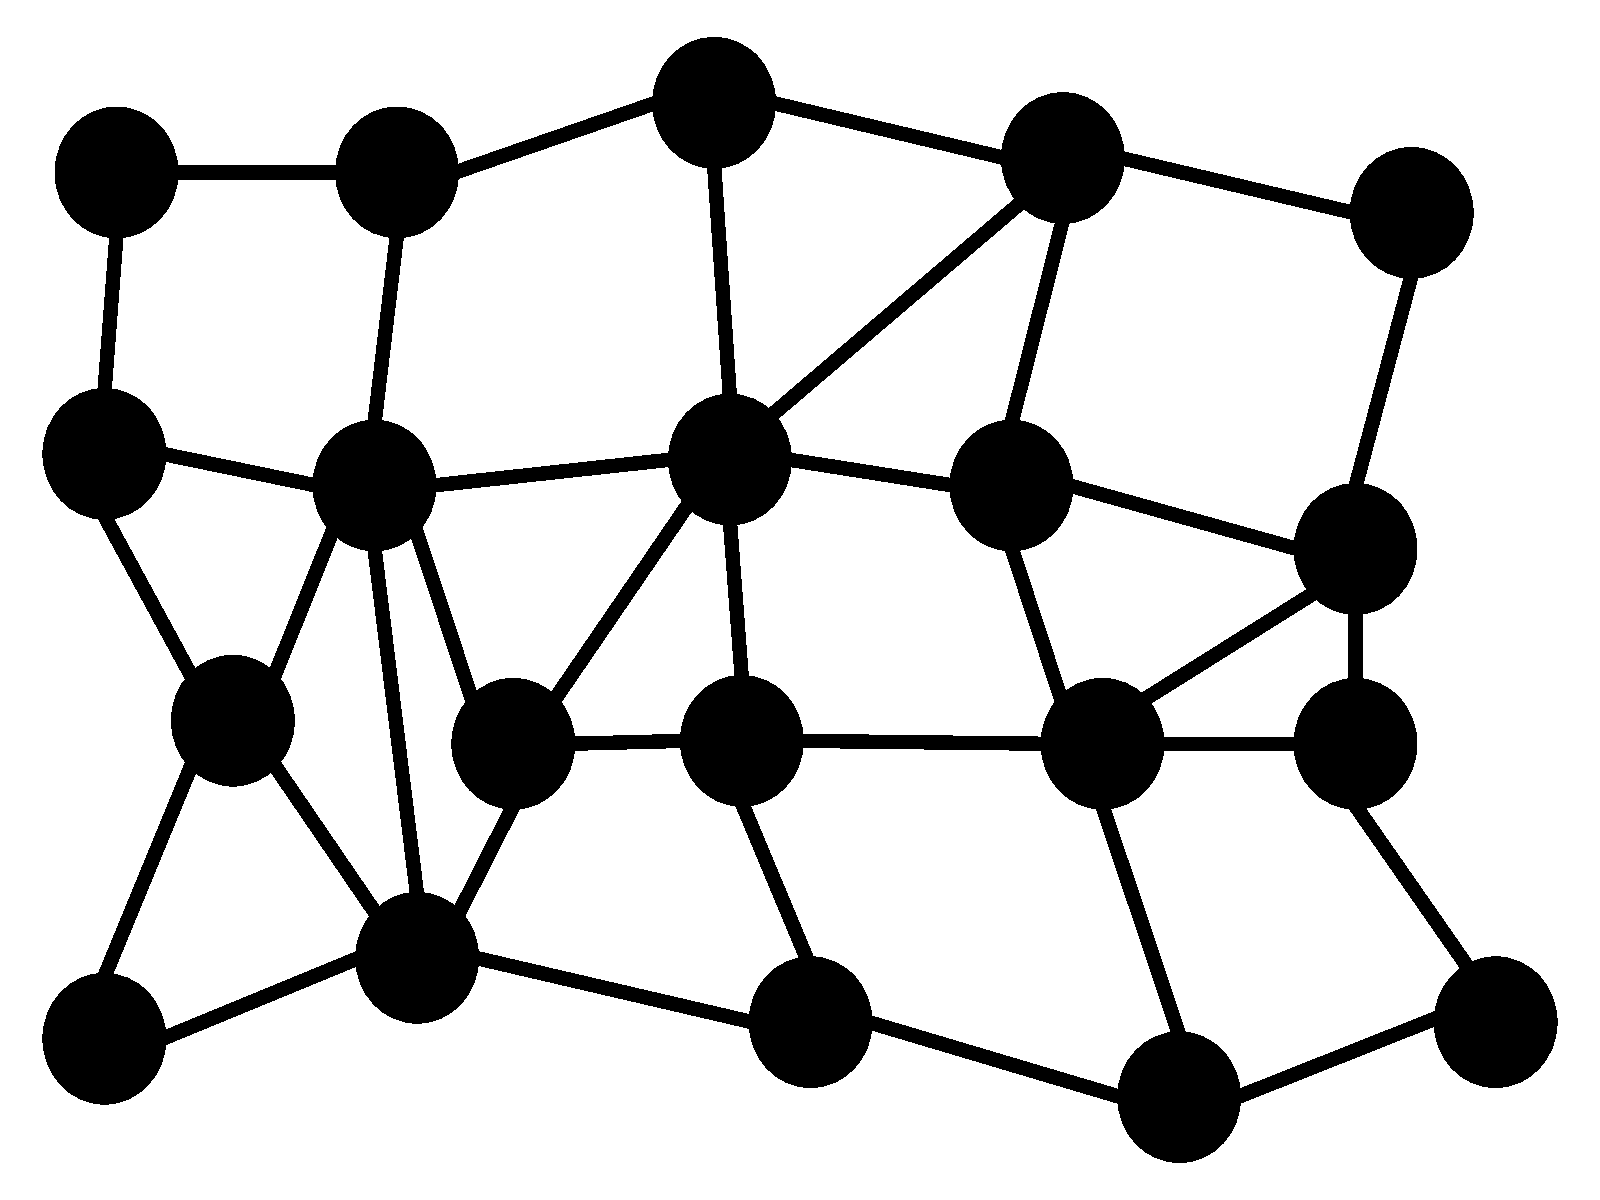
\includegraphics[clip=true, width=\textwidth]{Images/unstructured.pdf}
    \caption{unstructured}
    \label{fig:unstructured}
  \end{subfigure}
  \begin{subfigure}[b]{0.2\textwidth}
    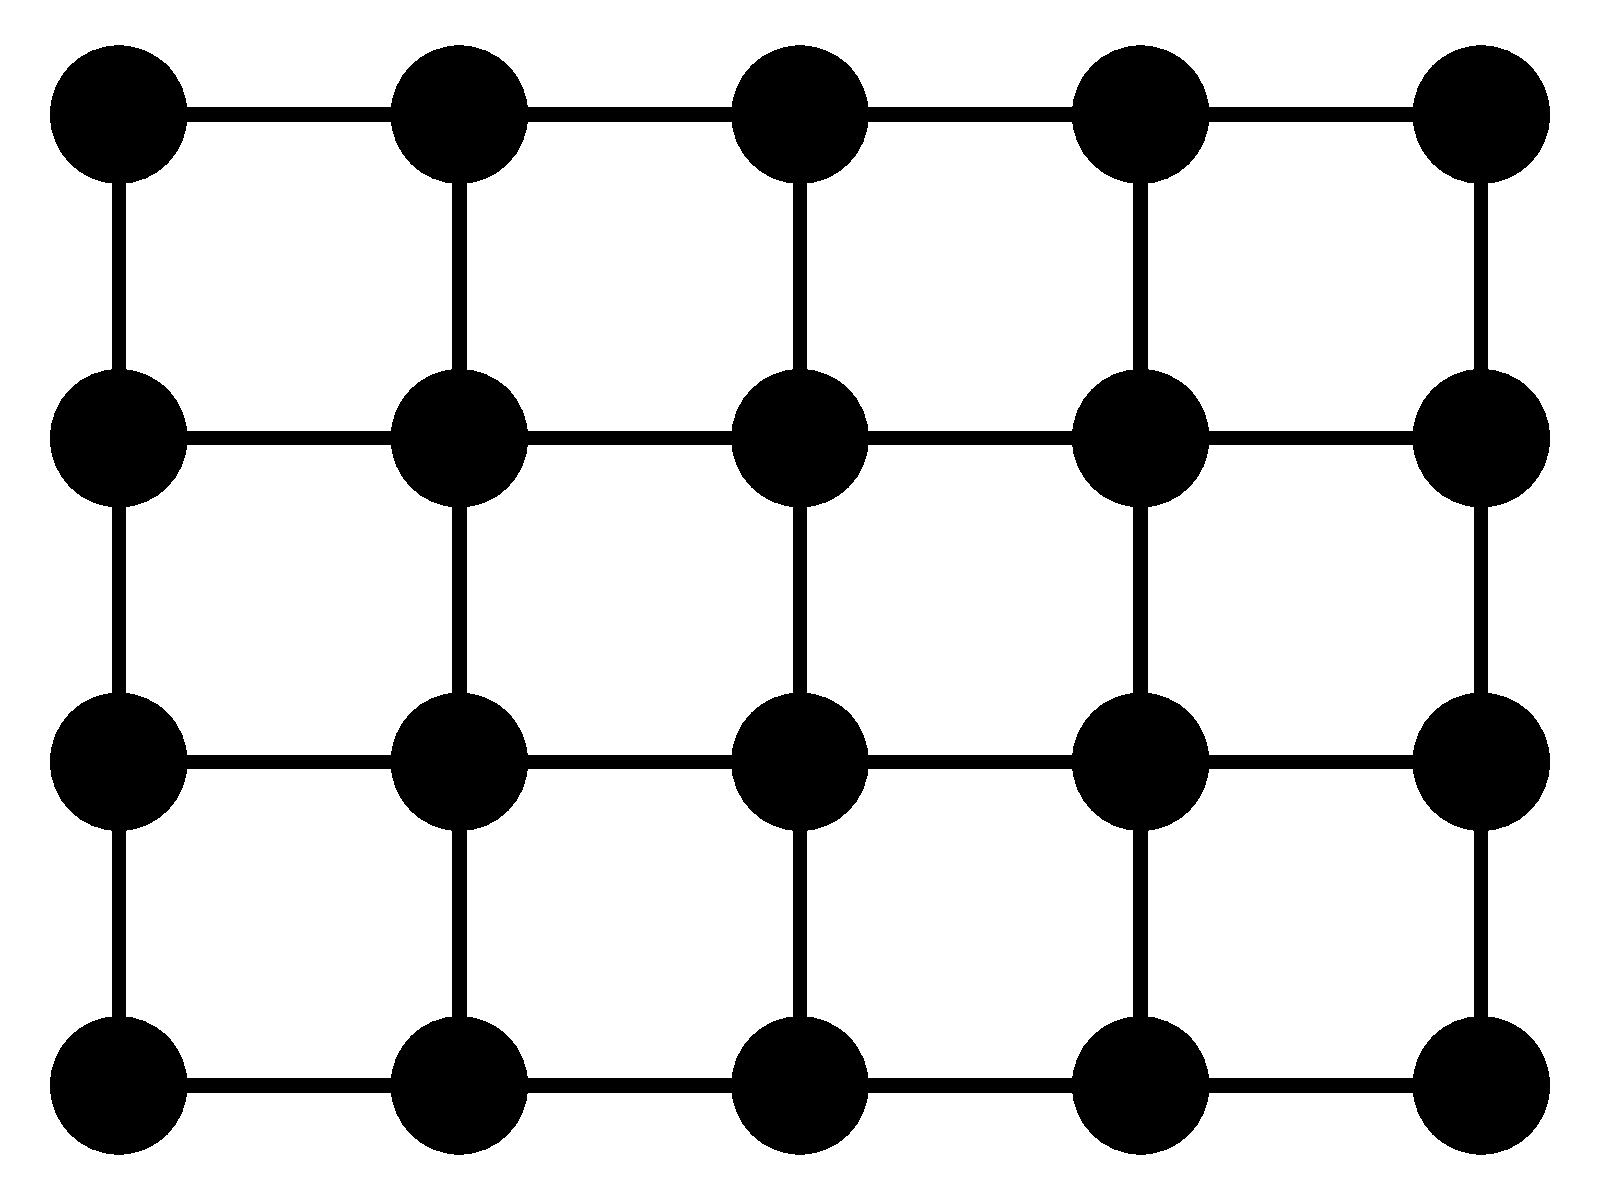
\includegraphics[clip=true, width=\textwidth]{Images/uniform.pdf}
    \caption{uniform}
    \label{fig:uniform}
  \end{subfigure}
  \begin{subfigure}[b]{0.2\textwidth}
    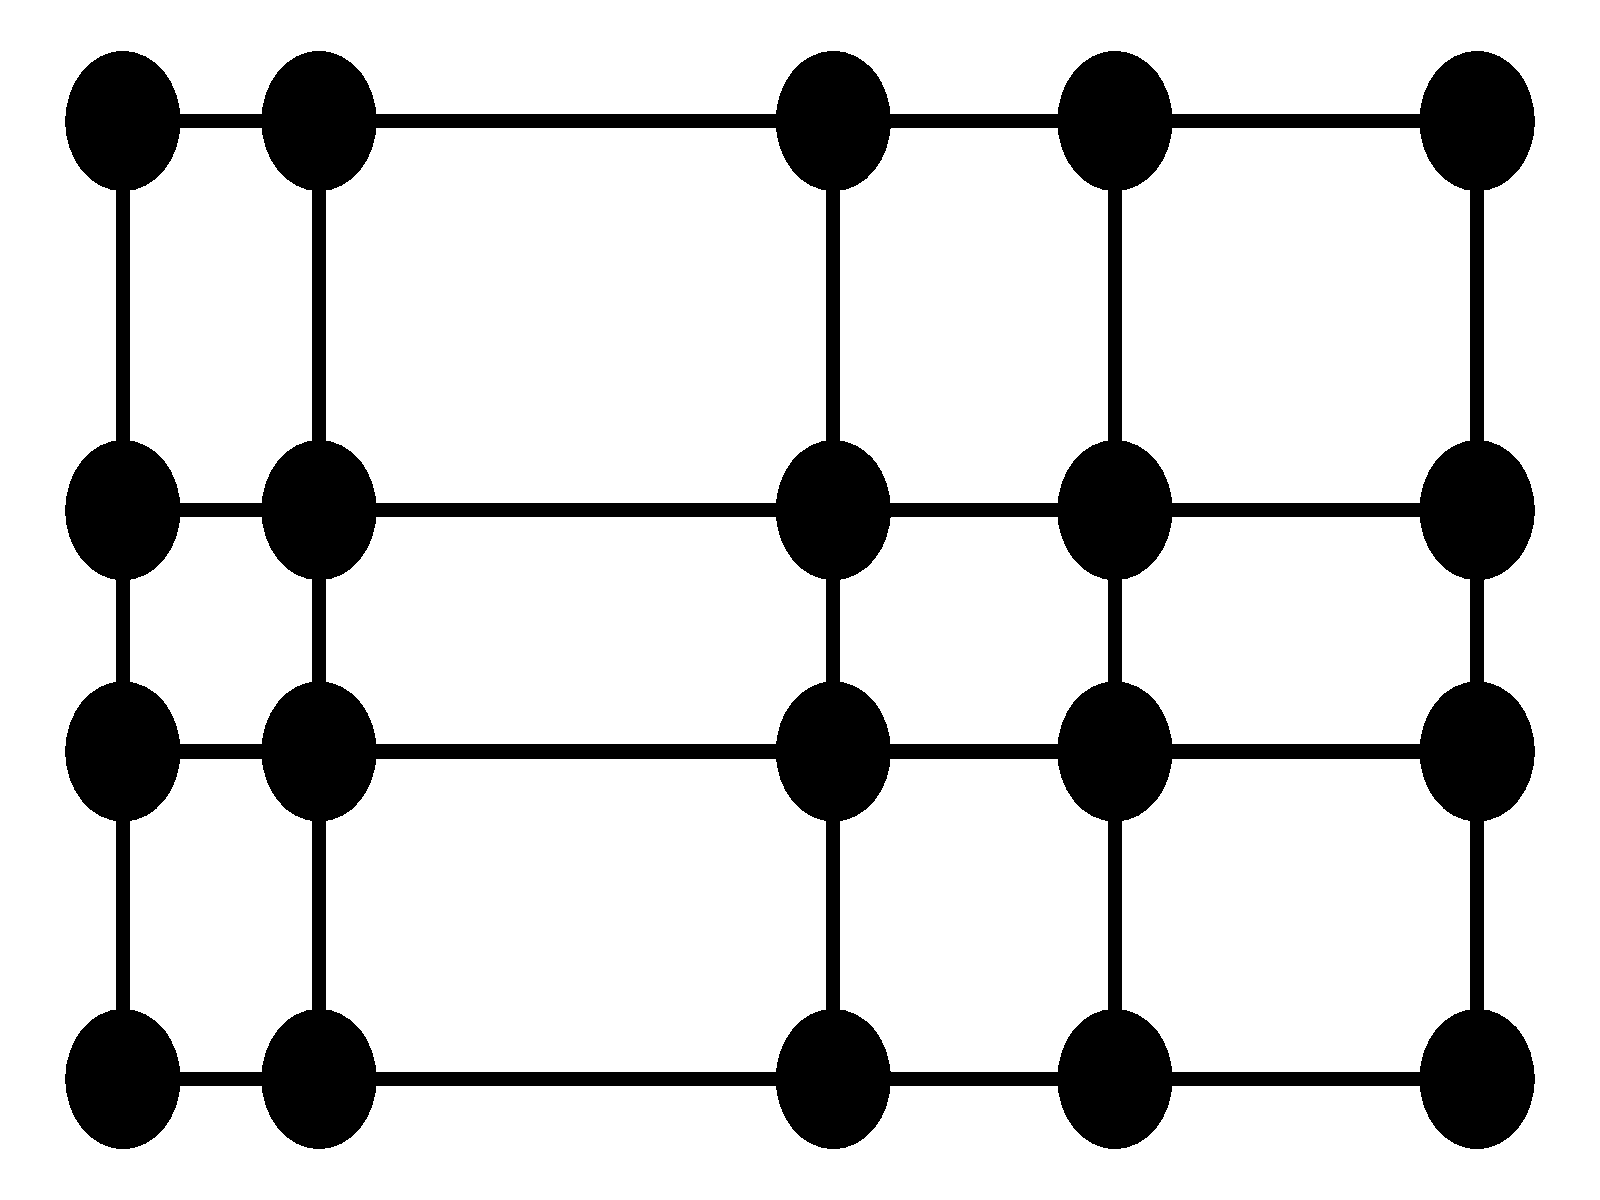
\includegraphics[clip=true, width=\textwidth]{Images/rectilinear.pdf}
    \caption{rectilinear}
    \label{fig:rectilinear}
  \end{subfigure}
  \begin{subfigure}[b]{0.19\textwidth}
    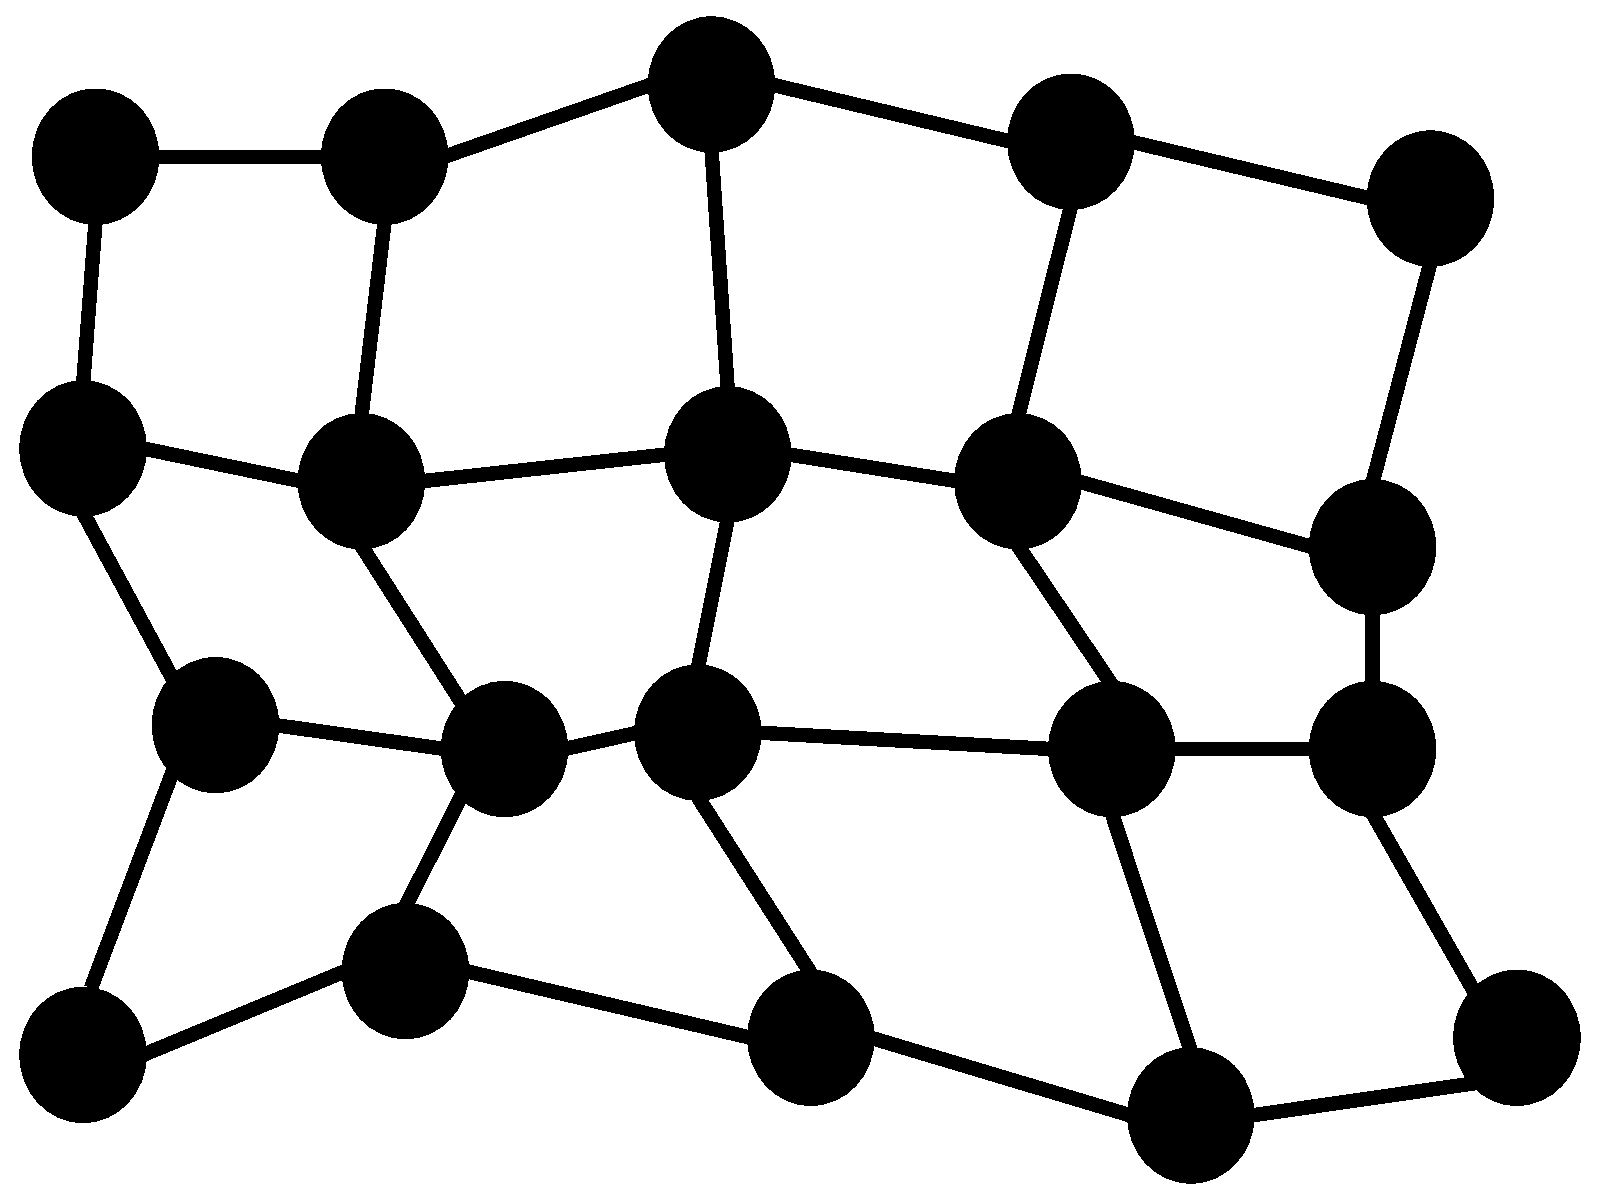
\includegraphics[clip=true, width=\textwidth]{Images/curvilinear.pdf}
    \caption{curvilinear}
    \label{fig:curvilinear}
  \end{subfigure}
  
  \caption{Different types of grids. Uniform structured grids like in
  Figure~\ref{fig:uniform} can have varying distances inbetween
  dimensions, but along a dimension, the distances of the nodes are
  equal. Figure~\ref{fig:uniform}, \ref{fig:rectilinear} and
  \ref{fig:curvilinear} are variants of structured grids and therefore
  their connectivity is given by the ordering of the nodes.}
  \label{fig:grids}
\end{figure}

%%%%%%%%%%%%%%%%%%%%%%%%%%%%%%%%%%%%%%%%%%%%%%%%%%%%%%%%%%%%%%%%%%%%%%%%
\section{Scalar Fields}
%%%%%%%%%%%%%%%%%%%%%%%%%%%%%%%%%%%%%%%%%%%%%%%%%%%%%%%%%%%%%%%%%%%%%%%%

An $n$-dimensional field with a single scalar value at every point in
space is called a scalar field. A simple example for a scalar field is a
height map of some geographical terrain. It has two dimensions with a
height value at every point encoded with color. In this work we will use
the notation $S(x)$ for the scalar value at point $x = (x_1,\dots,x_n)$
in the scalar field $S$ with $S: \real^n \rightarrow \real$. While in
continuous scalar fields the values of every point are defined by a
function, discrete scalar fields only have values at specific points in
space. As real world data is often acquired by measuring certain
locations and usually does not follow any graspable function, we will
focus on discrete scalar fields in this work, where $n \in \{2,3\}$.
This also applies to the other types of fields we will encounter,
because they have the same resolution as the scalar field.
\\(INSERT PICTURE OF HEIGHT MAP)

%%%%%%%%%%%%%%%%%%%%%%%%%%%%%%%%%%%%%%%%%%%%%%%%%%%%%%%%%%%%%%%%%%%%%%%%
\subsection{Uncertain Scalar Fields}\label{sec:USF}
%%%%%%%%%%%%%%%%%%%%%%%%%%%%%%%%%%%%%%%%%%%%%%%%%%%%%%%%%%%%%%%%%%%%%%%%

Unlike certain scalar fields, uncertain scalar fields have multiple
values for every point of the domain. Following the work of Theisel
\etal{\cite{Vortex}}, we assume that these values are Gaussian
distributed over the $m$ members of the data ensemble obtained from
simulations or measurements and therefore

\begin{equation}
  S_{\mathcal{N}}(x) = \mathcal{N}(\mu_{x}, \sigma_{x}^2),
\end{equation}

\noindent where $\mu_x$ is the mean scalar value and $\sigma_{x}^2$ the
variance of the $m$ entities at point $x = (x_1,\dots,x_n)$. As they
also pointed out in their work, we need to consider the neighborhood of
$x$, so that the derivatives of the uncertain scalar field are Gaussian
distributed as well. As we will explain in Chapter~\ref{chap:Method}, we
will search for ridges (Section~\ref{sec:Ridges}) inside cells.
Therefore, combining this with the need for neighboring points, we have
4 (or 8 in the 3D case) nodes of the cell we want to observe, together
with their neighboring points in every dimension and, because we also
want to calculate the second derivative, their neighboring nodes as
well. Cleared from redundant points, this results in 24 (80) nodes per
neighborhood as illustrated in Figure~\ref{fig:NH}. We can take this
neighborhood as a vector $v_x$ and calculate the $24$-dimensional mean
vector at point $x$ of the mean vector field $\mu(x) = \frac{1}{m}
\sum_{k=1}^m v_{x,k}$, followed by the $24 \times 24$-dimensional
covariance matrix, with the covariance field being $\Sigma(x)= \frac{1}{m}
\sum_{k=1}^m (v_{x,k} - \mu(x)){(v_{x,k} - \mu{(x)})}^\top$. Therefore our
uncertain scalar fields follows a multivariate Gaussian distribution
at every location

\begin{equation}
  S_{\mathcal{N}}(x) = \mathcal{N}(\mu(x), \Sigma(x)).\\
\end{equation}

\begin{figure}
  \centering
  \begin{subfigure}[b]{0.4\textwidth}
    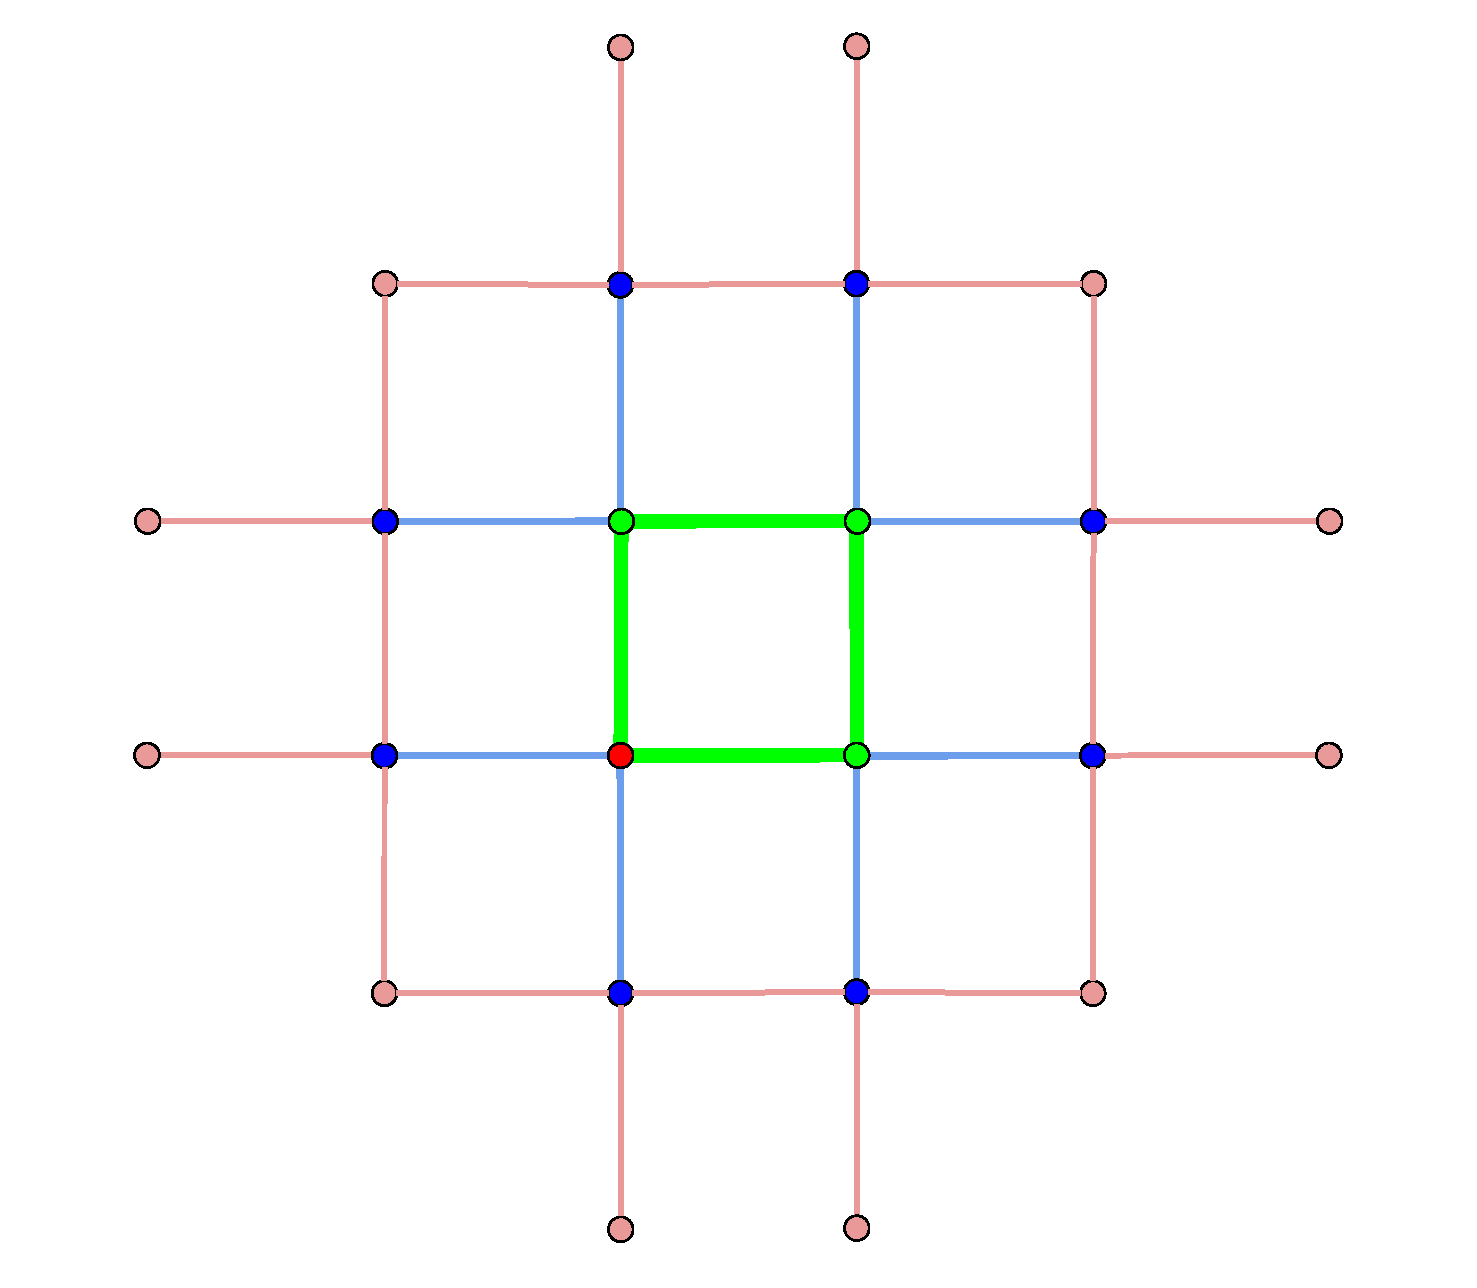
\includegraphics[width=\textwidth]{Images/2DNH.pdf}
    \caption{2D neighborhood}
    \label{fig:2DNH}
  \end{subfigure}
  \begin{subfigure}[b]{0.49\textwidth}
    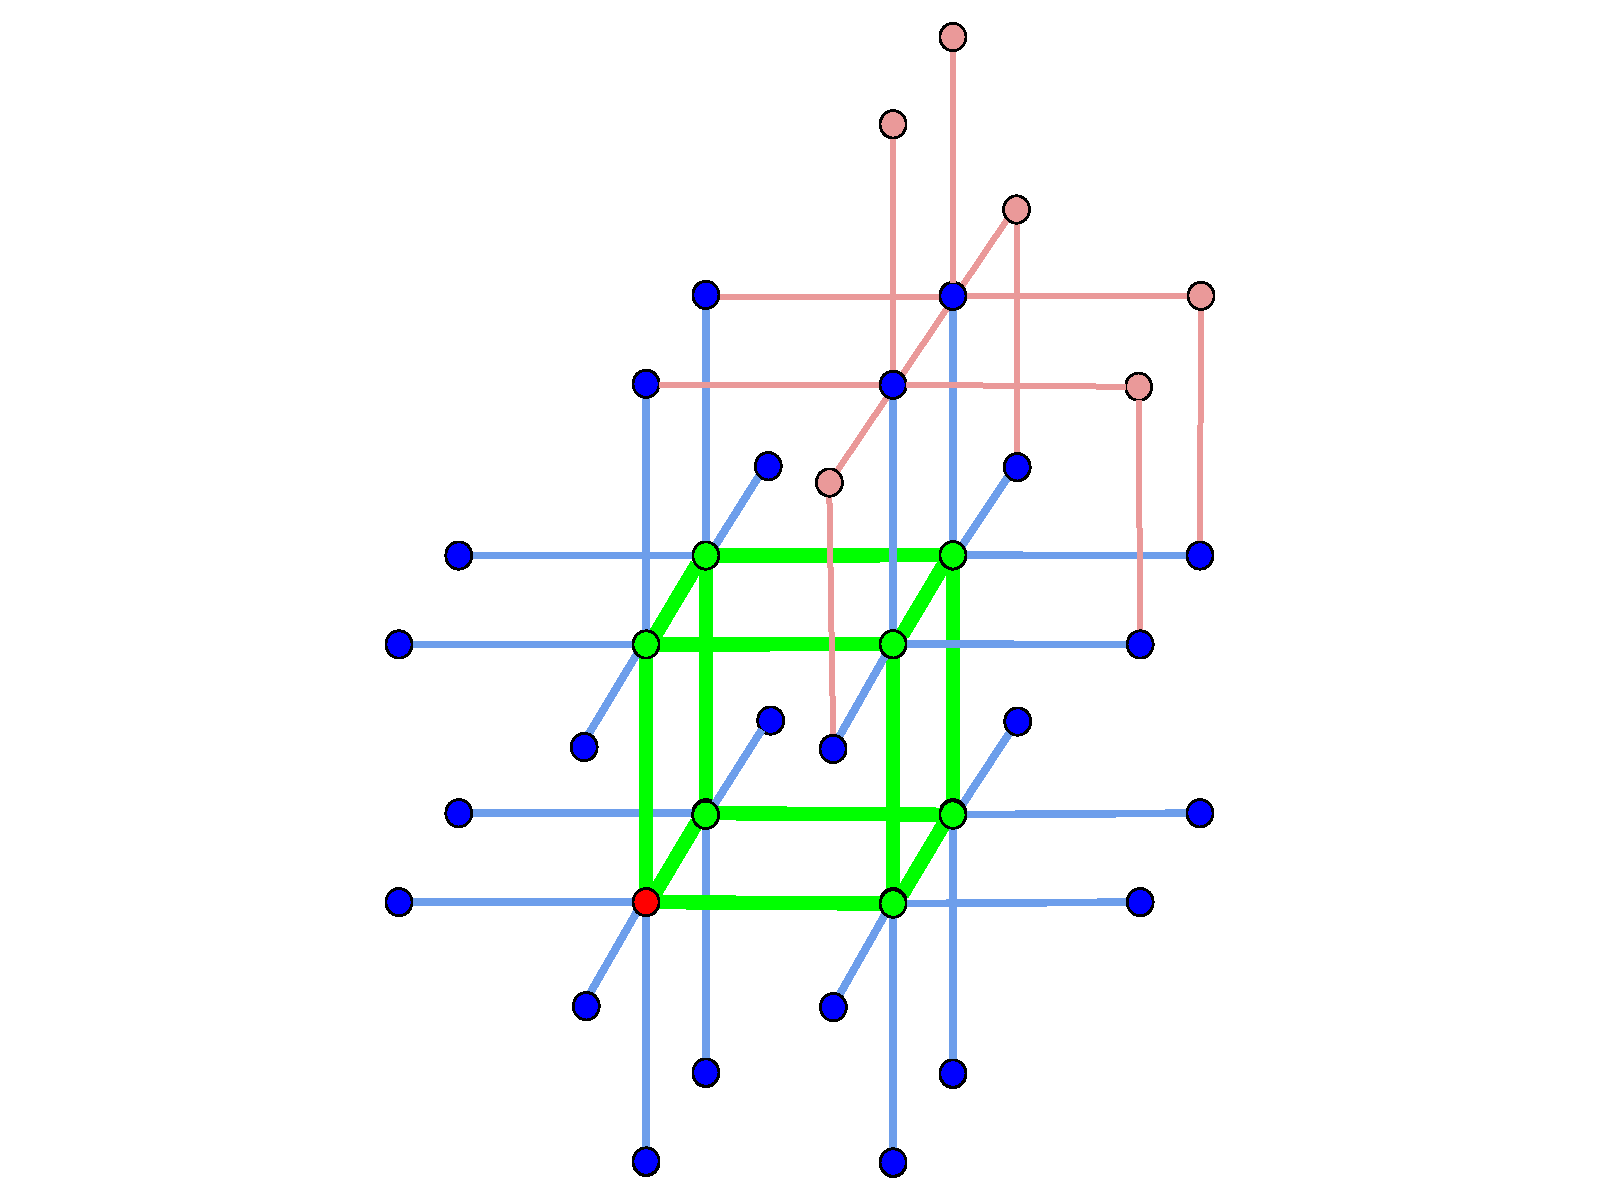
\includegraphics[width=\textwidth]{Images/3DNH.pdf}
    \caption{3D neighborhood}
    \label{fig:3DNH}
  \end{subfigure}
  \caption{Support regions for the 2- and 3-dimensional case. A cell of
  this size is created for every node of the initial scalar fields,
  depending on the dimensionality of the data set. The red node marks
  the location of the actual node at this position in the scalar field,
  the green nodes belong to the cell we want to inspect and the blue
  nodes are used to calculate the gradient of the green nodes via
  central differences, as well as the gradient of the red node of
  course. The outer pink nodes are used for the gradient of the blue
  ones and with their gradient we can estimate the Hessian
  matrices of the cell nodes. The neighboring points of the blue nodes
  in Figure~\ref{fig:3DNH} are only drawn for the two upper right ones,
  as drawing all of them would make the image too cluttered.}
  \label{fig:NH}
\end{figure}

%%%%%%%%%%%%%%%%%%%%%%%%%%%%%%%%%%%%%%%%%%%%%%%%%%%%%%%%%%%%%%%%%%%%%%%%
\section{Vector Fields}
%%%%%%%%%%%%%%%%%%%%%%%%%%%%%%%%%%%%%%%%%%%%%%%%%%%%%%%%%%%%%%%%%%%%%%%%

An $n$-dimensional vector field $V$ associates an $m$-dimensional vector
with every point in space $V(x_1,\dots,x_n):\real^n \rightarrow \real^m$.
If the vector field is the result of deriving a scalar field, thus the 
vector field is the gradient of the scalar field, the vector field is
called conservative. Conservative vector fields have the property, that
the line integral along any path connecting two points is always equal.
Since we are extracting features from scalar fields in this work, our
vector fields will always be conservative and $n = m$.

%%%%%%%%%%%%%%%%%%%%%%%%%%%%%%%%%%%%%%%%%%%%%%%%%%%%%%%%%%%%%%%%%%%%%%%%
\section{Tensor Fields}
%%%%%%%%%%%%%%%%%%%%%%%%%%%%%%%%%%%%%%%%%%%%%%%%%%%%%%%%%%%%%%%%%%%%%%%%

An $n$-dimensional tensor field $H$ associates an $l \times
m$-dimensional tensor with every point in space $H(x_1,\dots,x_n):
\real^n \rightarrow \real^{l \times m}$. Tensor fields are a
generalization of scalar and vector fields as a tensor with $l = m = 1$
would represent a scalar, and with $l > 1$ and $m = 1$ a vector. In our
case, the tensor field is a result of deriving a vector field, thus $n =
l = m$.

%%%%%%%%%%%%%%%%%%%%%%%%%%%%%%%%%%%%%%%%%%%%%%%%%%%%%%%%%%%%%%%%%%%%%%%%
\section{Derivatives}\label{sec:derivatives}
%%%%%%%%%%%%%%%%%%%%%%%%%%%%%%%%%%%%%%%%%%%%%%%%%%%%%%%%%%%%%%%%%%%%%%%%

Since we are dealing with discrete scalar fields, we have no function we
could derive to get the underlying gradient field. Instead we have to
approximate the derivatives with finite difference methods. There are
three forms which are commonly used:\\
\\
\begin{inparaenum}[(a)]
  \item Forward Differences
  \begin{equation}
    \nabla f(x_i) = \frac{f(x_{i+1}) - f(x_i)}{h}
  \end{equation}
  \item Backward Differences
  \begin{equation}
    \nabla f(x_i) = \frac{f(x_i) - f(x_{i-1})}{h}
  \end{equation}
  \item Central Differences
  \begin{equation}\label{eq:centDiff}
    \nabla f(x_i) = \frac{f(x_{i+1}) - f(x_{i-1})}{2h}
  \end{equation}
\end{inparaenum}
where $f(x_i)$ denotes the $i$-th point of the function $f(x): \real
\rightarrow \real$ and $h$ the distance between two neighboring points.
Forward and backward differences are used at the borders of the field,
where no previous or succeeding point is available. As we will explain
in Chapter~\ref{chap:Method}, with our current implementation we process
cells with a fixed size and therefore do not consider border cases, thus
this work focuses on central differences.

%----------------------------------------------------------------------%
\subsection{First Derivative}
%----------------------------------------------------------------------%

When deriving an $n$-dimensional scalar field $S$, we need to apply
Equation~\ref{eq:centDiff} for every dimension. This results in $n$
scalar values, representing the change of the scalar field in the
respective dimensions. These values can be interpreted as an
$n$-dimensional vector, pointing in the direction of greatest ascend for
every point of the scalar field. This is the gradient field $\nabla
S(x)$.

%----------------------------------------------------------------------%
\subsection{Second Derivative}
%----------------------------------------------------------------------%

The second derivative of an $n$-dimensional scalar field is an $n$
-dimensional tensor field with $\nabla^2 S:\real^n \rightarrow \real^{n
\times n}$. This tensor field can again be obtained with the central
difference method applied to every dimension of the gradient field. Here
we get an $n$-dimensional vector per dimension as we are subtracting the
previous gradient from the succeeding gradient of point $x$ along any
dimension. These vectors represent the respective columns of the so
called Hessian matrix. The Hessian matrix $H$ is a specification of the
Jacobian Matrix $J$, which derives any vector valued function $f(x):
\real^n \rightarrow \real^m$, $J \in \real^{m \times n}$. The Hessian
matrix is obtained when deriving a conservative vector field, therefore
the Hessian is quadratic with:

\begin{equation}
  H =
  \begin{bmatrix}
    \frac{\partial^2 S}{\partial x_1^2} & \frac{\partial^2 S}{\partial x_1 \partial x_2} & \dots & \frac{\partial^2 S}{\partial x_1 \partial x_n}\\
    \frac{\partial^2 S}{\partial x_2 \partial x_1} & \frac{\partial^2 S}{\partial x_2^2} & \dots & \frac{\partial^2 S}{\partial x_2 \partial x_n}\\
    \vdots & \vdots & \ddots & \vdots \\
    \frac{\partial^2 S}{\partial x_n \partial x_1} & \frac{\partial^2 S}{\partial x_n \partial x_2} & \dots & \frac{\partial^2 S}{\partial x_n^2}
  \end{bmatrix}
  \in \real^{n \times n}.
\end{equation}

\noindent According to Schwarz's theorem of the symmetry of second
derivatives ([ref]), the Hessian is assumed to be symmetric, therefore
the eigenvectors are orthogonal and the eigenvalues are real valued. The
eigenvalues of the Hessian denote the second directional derivative of
the scalar field along the direction of the corresponding eigenvector,
and thus the change of the gradient in the direction of the eigenvector.
\\(EXAMPLE?!)

%%%%%%%%%%%%%%%%%%%%%%%%%%%%%%%%%%%%%%%%%%%%%%%%%%%%%%%%%%%%%%%%%%%%%%%%
\section{Linear Interpolation}
%%%%%%%%%%%%%%%%%%%%%%%%%%%%%%%%%%%%%%%%%%%%%%%%%%%%%%%%%%%%%%%%%%%%%%%%

Our discrete fields only provide information for a limited number of
points along a dimension, therefore we need to estimate the values lying
between the known locations. To ease computation we assume that the
underlying functions of the fields are linear and apply linear
interpolation to the tensors $A, B \in \real^{n \times n}$ at the
neighboring points, independent of dimensionality. As we will explain in
Chapter~\ref{chap:Method}, we only apply interpolation on the edges of
cells and can therefore assume the distance between the two nodes to be
$1$. This leads to the interpolated tensor:

\begin{equation}
  T_{ipol} =
  \begin{bmatrix}
    (1-t) \cdot A_{11} + t \cdot B_{11} & \dots & (1-t) \cdot A_{1n} + t \cdot B_{1n} \\
    \vdots & \ddots & \vdots \\
    (1-t) \cdot A_{n1} + t \cdot B_{n1} & \dots & (1-t) \cdot A_{nn} + t \cdot B_{nn} \\
  \end{bmatrix}
  \in \real^{n \times n}
\end{equation}
with $t$ being the relative distance of the desired location to tensor
$A$. (see Figure ipol) We will only consider the cases for $n \in
\{1,2,3\}$.
\\(Picture explaining linear interpolation)

%%%%%%%%%%%%%%%%%%%%%%%%%%%%%%%%%%%%%%%%%%%%%%%%%%%%%%%%%%%%%%%%%%%%%%%%
\section{Matrix Decompositions}
%%%%%%%%%%%%%%%%%%%%%%%%%%%%%%%%%%%%%%%%%%%%%%%%%%%%%%%%%%%%%%%%%%%%%%%%

A matrix decomposition is a factorization of a matrix into its
constituent parts. In general there are two classes of factorizations:
decompositions used for solving linear equations and decompositions
based on eigenvalues and vectors. We will consider one example from each
class, namely the Cholesky and the Eigendecomposition. As we will
explain in Section~\ref{sec:MGS} we will use both decompositions to
generate samples from a multivariate gaussian distribution, even though
they are from different classes.

%----------------------------------------------------------------------%
\subsection{Cholesky Decomposition}\label{sec:cholesky}
%----------------------------------------------------------------------%

The Cholesky factorization is a decomposition of a square, hermititan,
positive definite matrix $A$ into the product of a lower-triangular
matrix L and its conjugate transpose $A = L L^*$. A matrix $C$ is
hermitian if the diagonal elements are real valued and $C_{ij} =
\overline{C_{ji}}$, meaning that $\overline{C_{ji}}$ is the complex
conjugate of $C_{ij}$. Two complex numbers are complex conjugate if they
have equal real and imaginary parts, but opposite signs. For example,
$1+i$ is the complex conjugate of $1-i$. Following this property, the
standard Cholesky decomposition is also applicable for every real
valued, symmetric, positive definite matrix, resulting in a lower
triangular real valued matrix and its transpose $A = L L^\top$. We
will only deal with real valued matrices in this work and therefore
follow this notation. A simple way to determine the definiteness of a
matrix is to look at its eigenvalues. If every eigenvalue $\lambda$ of a
square $n \times n$ matrix is greater than zero, $\lambda_{i} > 0, i \in
\{1,\dots,n\}$, the matrix is positive definite. If every eigenvalue is
greater or equal to zero, $\lambda_{i} \ge 0$, the matrix is positive
semi-definite. The same goes for negative eigenvalues, as they make the
matrix negative (semi-) definite.

%----------------------------------------------------------------------%
\subsubsection{$LDL^T$ Decomposition}
%----------------------------------------------------------------------%

The closely related $LDL^T$ decomposition extends the classical Cholesky
decomposition to semi-definite and negative definite matrices $A = L D
L^\top$, where $L$ is a lower unitriangular matrix, meaning there are
only ones on the diagonal, and $D$ is a diagonal matrix. The two
decompositions are related as follows:

\begin{equation}\label{eq:LDL}
  A = LDL^\top = (L D^\frac{1}{2}) (D^\frac{1}{2}  L^\top).
\end{equation}

\noindent This version has the advantage that it avoids extracting
square roots, thus allowing for negative entries in $D$, as it is
possible for some indefinite matrices for which no classical
decomposition exists, while having the same computational complexity as
the Cholesky decomposition. If the solution of a linear system is needed
and the system can be put into a symmetric form, the Cholesky
decomposition and its variant is the method of choice, as it offers
efficiency and usually numerical stability. Here is an example for both
variants of the decomposition:\\
\begin{inparaenum}[]
  \item Cholesky decomposition of a symmetric real valued matrix
  \begin{equation}
    \begin{pmatrix}
      9 & 18 & -27\\
      18 & 40 & -18 \\
      -27 & -18 & 406
    \end{pmatrix}
    =
    \begin{pmatrix}
      3 & 0 & 0\\
      6 & 2 & 0 \\
      -9 & 18 & 1
    \end{pmatrix}
    \begin{pmatrix}
      3 & 6 & -9\\
      0 & 2 & 18 \\
      0 & 0 & 1
    \end{pmatrix}
  \end{equation}
  \item $LDL^T$ decomposition of the same matrix
  \begin{equation}
    \begin{pmatrix}
      9 & 18 & -27\\
      18 & 40 & -18 \\
      -27 & -18 & 406
    \end{pmatrix}
    =
    \begin{pmatrix}
      1 & 0 & 0\\
      2 & 1 & 0 \\
      -3 & 9 & 1
    \end{pmatrix}
    \begin{pmatrix}
      9 & 0 & 0\\
      0 & 4 & 0 \\
      0 & 0 & 1
    \end{pmatrix}
    \begin{pmatrix}
      1 & 2 & -3\\
      0 & 1 & 9 \\
      0 & 0 & 1
    \end{pmatrix}
    .
  \end{equation}
\end{inparaenum}

%----------------------------------------------------------------------%
\subsection{Eigendecomposition}\label{sec:eigen}
%----------------------------------------------------------------------%

The Eigendecomposition is a factorization of a square $n \times n$,
diagonizable matrix $A$, into the form $A = E \Lambda E^{-1}$, where the
columns of $E$ are $n$ linearly independent eigenvectors of $A$ and
$\Lambda$ is a diagonal matrix with the respective eigenvalues. The
eigenvalue $\lambda_i$ at $\Lambda_{ii}$ corresponds to the eigenvector
$\epsilon_i$ at column $i, i \in \{1,\dots,n\}$ of $E$. This follows the
basic attribute of eigenvectors, as they only change by a scalar factor
when multiplied with their respective matrix, meaning $A \epsilon =
\lambda \epsilon$ and therefore $A E = E \Lambda$, which leads to the
decomposition $A = E \Lambda E^{-1}$. Here is a simple example of the
Eigendecomposition of a symmetric, real, diagonizable matrix:

\begin{equation}
  \begin{pmatrix}
    1 & {-3} & 3\\
    3 & {-5} & 3\\
    6 & {-6} & 4
  \end{pmatrix}
  =
  \begin{pmatrix}
    1 & {-1} & 1\\
    1 & 0 & 1\\
    2 & 1 & 0
  \end{pmatrix}
  \begin{pmatrix}
    4 & 0 & 0\\
    0 & {-2} & 0\\
    0 & 0 & {-2}
  \end{pmatrix}
  \begin{pmatrix}
    0.5 & {-0.5} & 0.5\\
    {-1} & 1 & 0\\
    {-0.5} & 1.5 & {-0.5}
  \end{pmatrix}
  .
\end{equation}

\noindent An $n \times n$-dimensional matrix is diagonizable if it has
$n$ linearly independent eigenvectors. The decomposition can for example
be used to easily raise a matrix to a power, as you only have to raise
the eigenvalue matrix $\Lambda$ to that power:

\begin{equation}
  \begin{pmatrix}
    1 & {-3} & 3\\
    3 & {-5} & 3\\
    6 & {-6} & 4
  \end{pmatrix}
  ^4
  =
  E
  \Lambda^4
  E^{-1}
  =
  \begin{pmatrix}
    136 & {-120} & 120\\
    120 & {-104} & 120\\
    240 & {-240} & 256
  \end{pmatrix}
  .
\end{equation}

\noindent In this work, our matrices don't need to be diagonizable, as
this property is only required for the inverse of the eigenvector
matrix. Section~\ref{sec:MGS} will give more information on that matter.


%----------------------------------------------------------------------%
\subsubsection{Principal Component Analysis}
%----------------------------------------------------------------------%

Even though the Principal Component Analysis (PCA) is not a decomposition
in itself, it is an application of the Eigendecomposition. In general,
the PCA fits an $n$-dimensional ellipsoid around a set of possibly
correlated points. The first principle component then corresponds to the
axis of biggest magnitude of the ellipsoid and therefore the axis of the
largest variance of the data. The principal components are always
orthogonal to each other. When the Eigendecomposition is applied to
a matrix containing correlated points, the resulting eigenvectors match
the principal components, and the eigenvalues the variance along those
axes. See Figure~\ref{fig:PCA} for a graphical example.

\begin{figure}
  \centering
  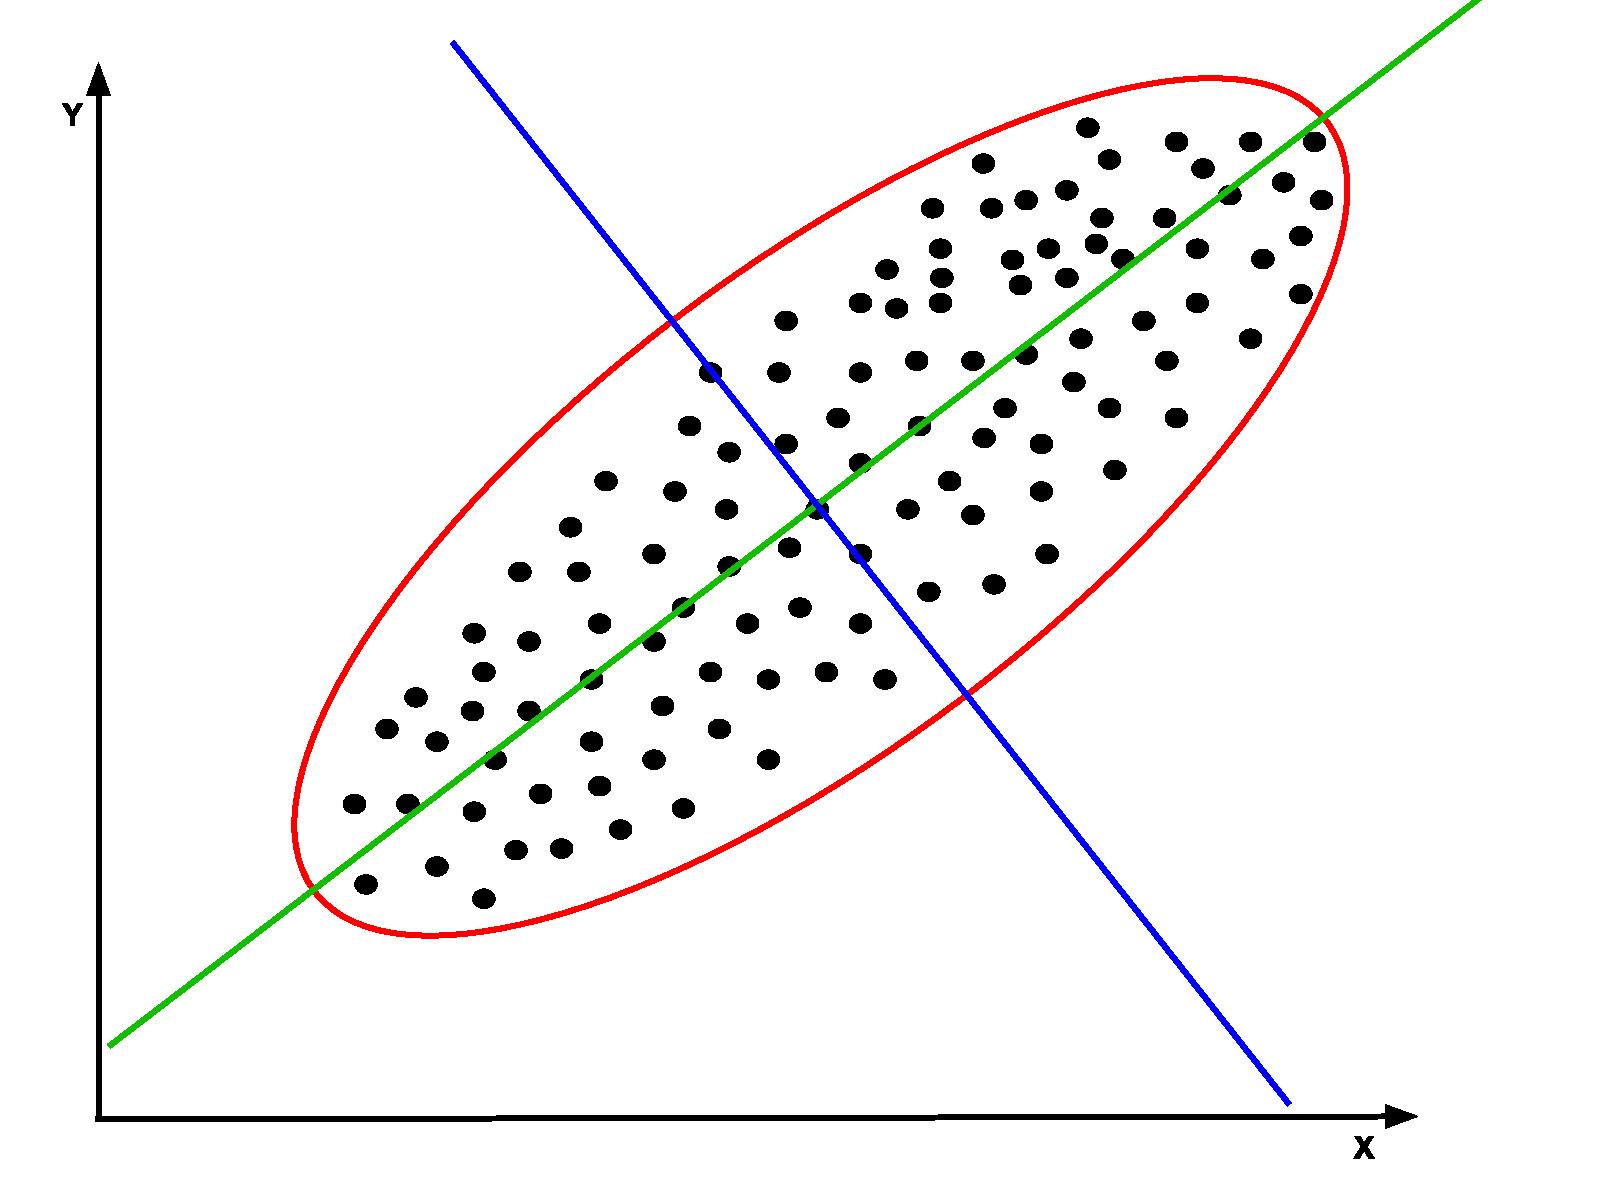
\includegraphics[width=0.75\textwidth]{Images/PCA.pdf}
  \caption{Principal Component Analysis of a set of points in
  $2$-dimensional space. The green line denotes the line of greatest
  variance, whereas the blue line is orthogonal to the green one and
  goes along the least variance. These lines correspond to the
  eigenvectors of a matrix containing the $x$ and $y$ coordinates of the
  points as columns.}
  \label{fig:PCA}
\end{figure}

%%%%%%%%%%%%%%%%%%%%%%%%%%%%%%%%%%%%%%%%%%%%%%%%%%%%%%%%%%%%%%%%%%%%%%%%
\section{Box-Muller Transformation}\label{sec:BM}
%%%%%%%%%%%%%%%%%%%%%%%%%%%%%%%%%%%%%%%%%%%%%%%%%%%%%%%%%%%%%%%%%%%%%%%%

The Box-Muller Transformation is a method to transform two uniformly
distributed random numbers into two independent, standard, normally
distributed random numbers. Let $U_1$ and $U_2$ be samples from the
uniform distribution on the interval ($0$, $1$). Let $N_1$ and $N_2$ be:

\begin{align}
  &N_1 = \sqrt{-2 \ln{U_1}} \cos (2 \pi U_2) \\
  &N_2 = \sqrt{-2 \ln{U_1}} \sin (2 \pi U_2).
\end{align}

\noindent Then $N_1$ and $N_2$ are independent random numbers with a
standard normal distribution, meaning that their mean is $\mu = 0$ and
standard deviation $\sigma = 1$. This transformation can be repeated to
generate standard normal distributed vectors of arbitrary length.

%%%%%%%%%%%%%%%%%%%%%%%%%%%%%%%%%%%%%%%%%%%%%%%%%%%%%%%%%%%%%%%%%%%%%%%%
\section{Ridges}\label{sec:Ridges}
%%%%%%%%%%%%%%%%%%%%%%%%%%%%%%%%%%%%%%%%%%%%%%%%%%%%%%%%%%%%%%%%%%%%%%%%

While the intuitive definition of a ridge would be a path along the
crest of a mountain with terrain falling off on either side, we focus on
a mathematical definition of ridges. In principal, a ridge is a local
maximum of an $n$-dimensional function. The maximum of the
$1$-dimensional function $f(x) = -x^2$ would be the $0$-dimensional
point at $x=0$, the ridge point (INSERT REF). When we add a dimension,
the domain becomes a $2$-dimensional surface, and the ridge point
expands into a $1$-dimensional ridge line (INSERT REF). Adding another
dimension turns the function domain into a $3$-dimensional volume and
the ridge into a $2$-dimensional surface (INSERT REF). In general, the
ridge is an $n-k$-dimensional manifold in an $n$-dimensional space for
$k=\{1, \dots, n\}$. This means that ridge points and lines also exist
in $3$-dimensional domains for example. This work focuses on ridges in
$2$ and $3$-dimensional domains.\\
To calculate the maximum, we need to derive the function and search for
the points where the derived function is $0$. The derived function
$f'(x)=-2x$ has only one zero at $x=0$. Now we only know that we have
found an extremum and need to check whether its a maximum or minimum by
looking at the second derivative $f''(x)=-2$. As $-2 < 0$, we now know
that the extremum is a maximum. The same principal is applicable for
ridges in higher dimensions. Here the first derivative at point $x$, the
gradient, lies in the subspace spanned by $n-k$ eigenvectors of the
Hessian, the second derivative, if $x$ is on an $n-k$ dimensional ridge.
In other words, the dot product of the gradient with the remaining $k$
eigenvectors is $0$, as the dot product is the scalar projection of two
vectors or a measurement for how much the gradient points into the
direction of the eigenvector. Keep in mind that the gradient always
points into the direction of greatest ascend. These eigenvectors
therefore have to be orthogonal to the gradient and the corresponding
eigenvalues have to be negative just like in the example above, as $x$
is a maximum along the directions of the $k$ eigenvectors, thus falls
off in their directions and only increases along the direction of the
$n-k$ eigenvectors. Figure~(INSERT REF) explains this connection on a
simple two dimensional example. The question remaining is how to decide
which eigenvectors denote the ridge domain. Eberly~\cite{Eberly} and
Lindeberg~\cite{Lindeberg} proposed two ways on how to sort the
eigenvalues $\lambda_i$ in order to pick the right corresponding
eigenvectors $\epsilon_i$:\\
\begin{inparaenum}[]
  \item Eberly
  \begin{equation}\label{eq:Eberly}
   \lambda_1 \leq \cdots \leq \lambda_n
  \end{equation}
  \item Lindeberg
  \begin{equation}
    \lvert \lambda_1 \rvert \geq \cdots \geq \lvert \lambda_n \rvert.
  \end{equation}
\end{inparaenum}
\noindent Lindebergs method extracts a subset of the ridge features
found by Eberly. Lindeberg discards a feature if there is along any
eigenvector an upward bend, denoted by a positive eigenvalue, that is
stronger than the downward bend along the $n-k$ eigenvectors found by
Eberly. For the definition of Eberly, an upward bend along the ridge is
irrelevant for its existence. This work will use Eberlys method and
therefore the principle definition for the existence of an $n-k$
dimensional ridge at point $x \in \real^n$ is:\\

\begin{equation}\label{eq:ridgeDot}
  \nabla S(x) \cdot \epsilon_1 = \cdots = \nabla S(x) \cdot \epsilon_{k} = 0
\end{equation}
\begin{equation}\label{eq:ridgeEV}
  \lambda_k < 0
\end{equation}

\noindent The counterpart to ridges are valleys. These can be obtained
by extracting ridges from the scalar field $-S(x)$ or by checking
Equation~\ref{eq:ridgeDot} for the eigenvectors corresponding to the
$k$ largest eigenvalues and $\lambda_k > 0$.
\\(PICTURES FOR RIDGE TYPES)

%%%%%%%%%%%%%%%%%%%%%%%%%%%%%%%%%%%%%%%%%%%%%%%%%%%%%%%%%%%%%%%%%%%%%%%%
\section{Marching Cubes}
%%%%%%%%%%%%%%%%%%%%%%%%%%%%%%%%%%%%%%%%%%%%%%%%%%%%%%%%%%%%%%%%%%%%%%%%

The Marching Cubes algorithm~\cite{MC} is a method to extract
isosurfaces from 3-dimensional discrete scalar fields. It got its name
due to the cell-wise extraction of the isosurface. The first step of the
algorithm is to check whether the nodes of the examined cell are either
below or above the desired isovalue. After that, a lookup table is
consulted that gives information on which edges of the cell connect such
two nodes. If every value is above or below the isovalue, the cell does
not contain a surface. Now linear interpolation is used to find the
location of the isosurface on the respective edges and the found points
are vertices of a triangle meshes. Figure~\ref{fig:MCTable} shows the
15 unique configurations for a surface in the cell, without
rotated variants. The same principle is used for the two dimensional
version, the Marching Squares algorithm. In that case the lookup table
is a lot simpler, as there are only four edges to check.

\begin{figure}
  \centering
  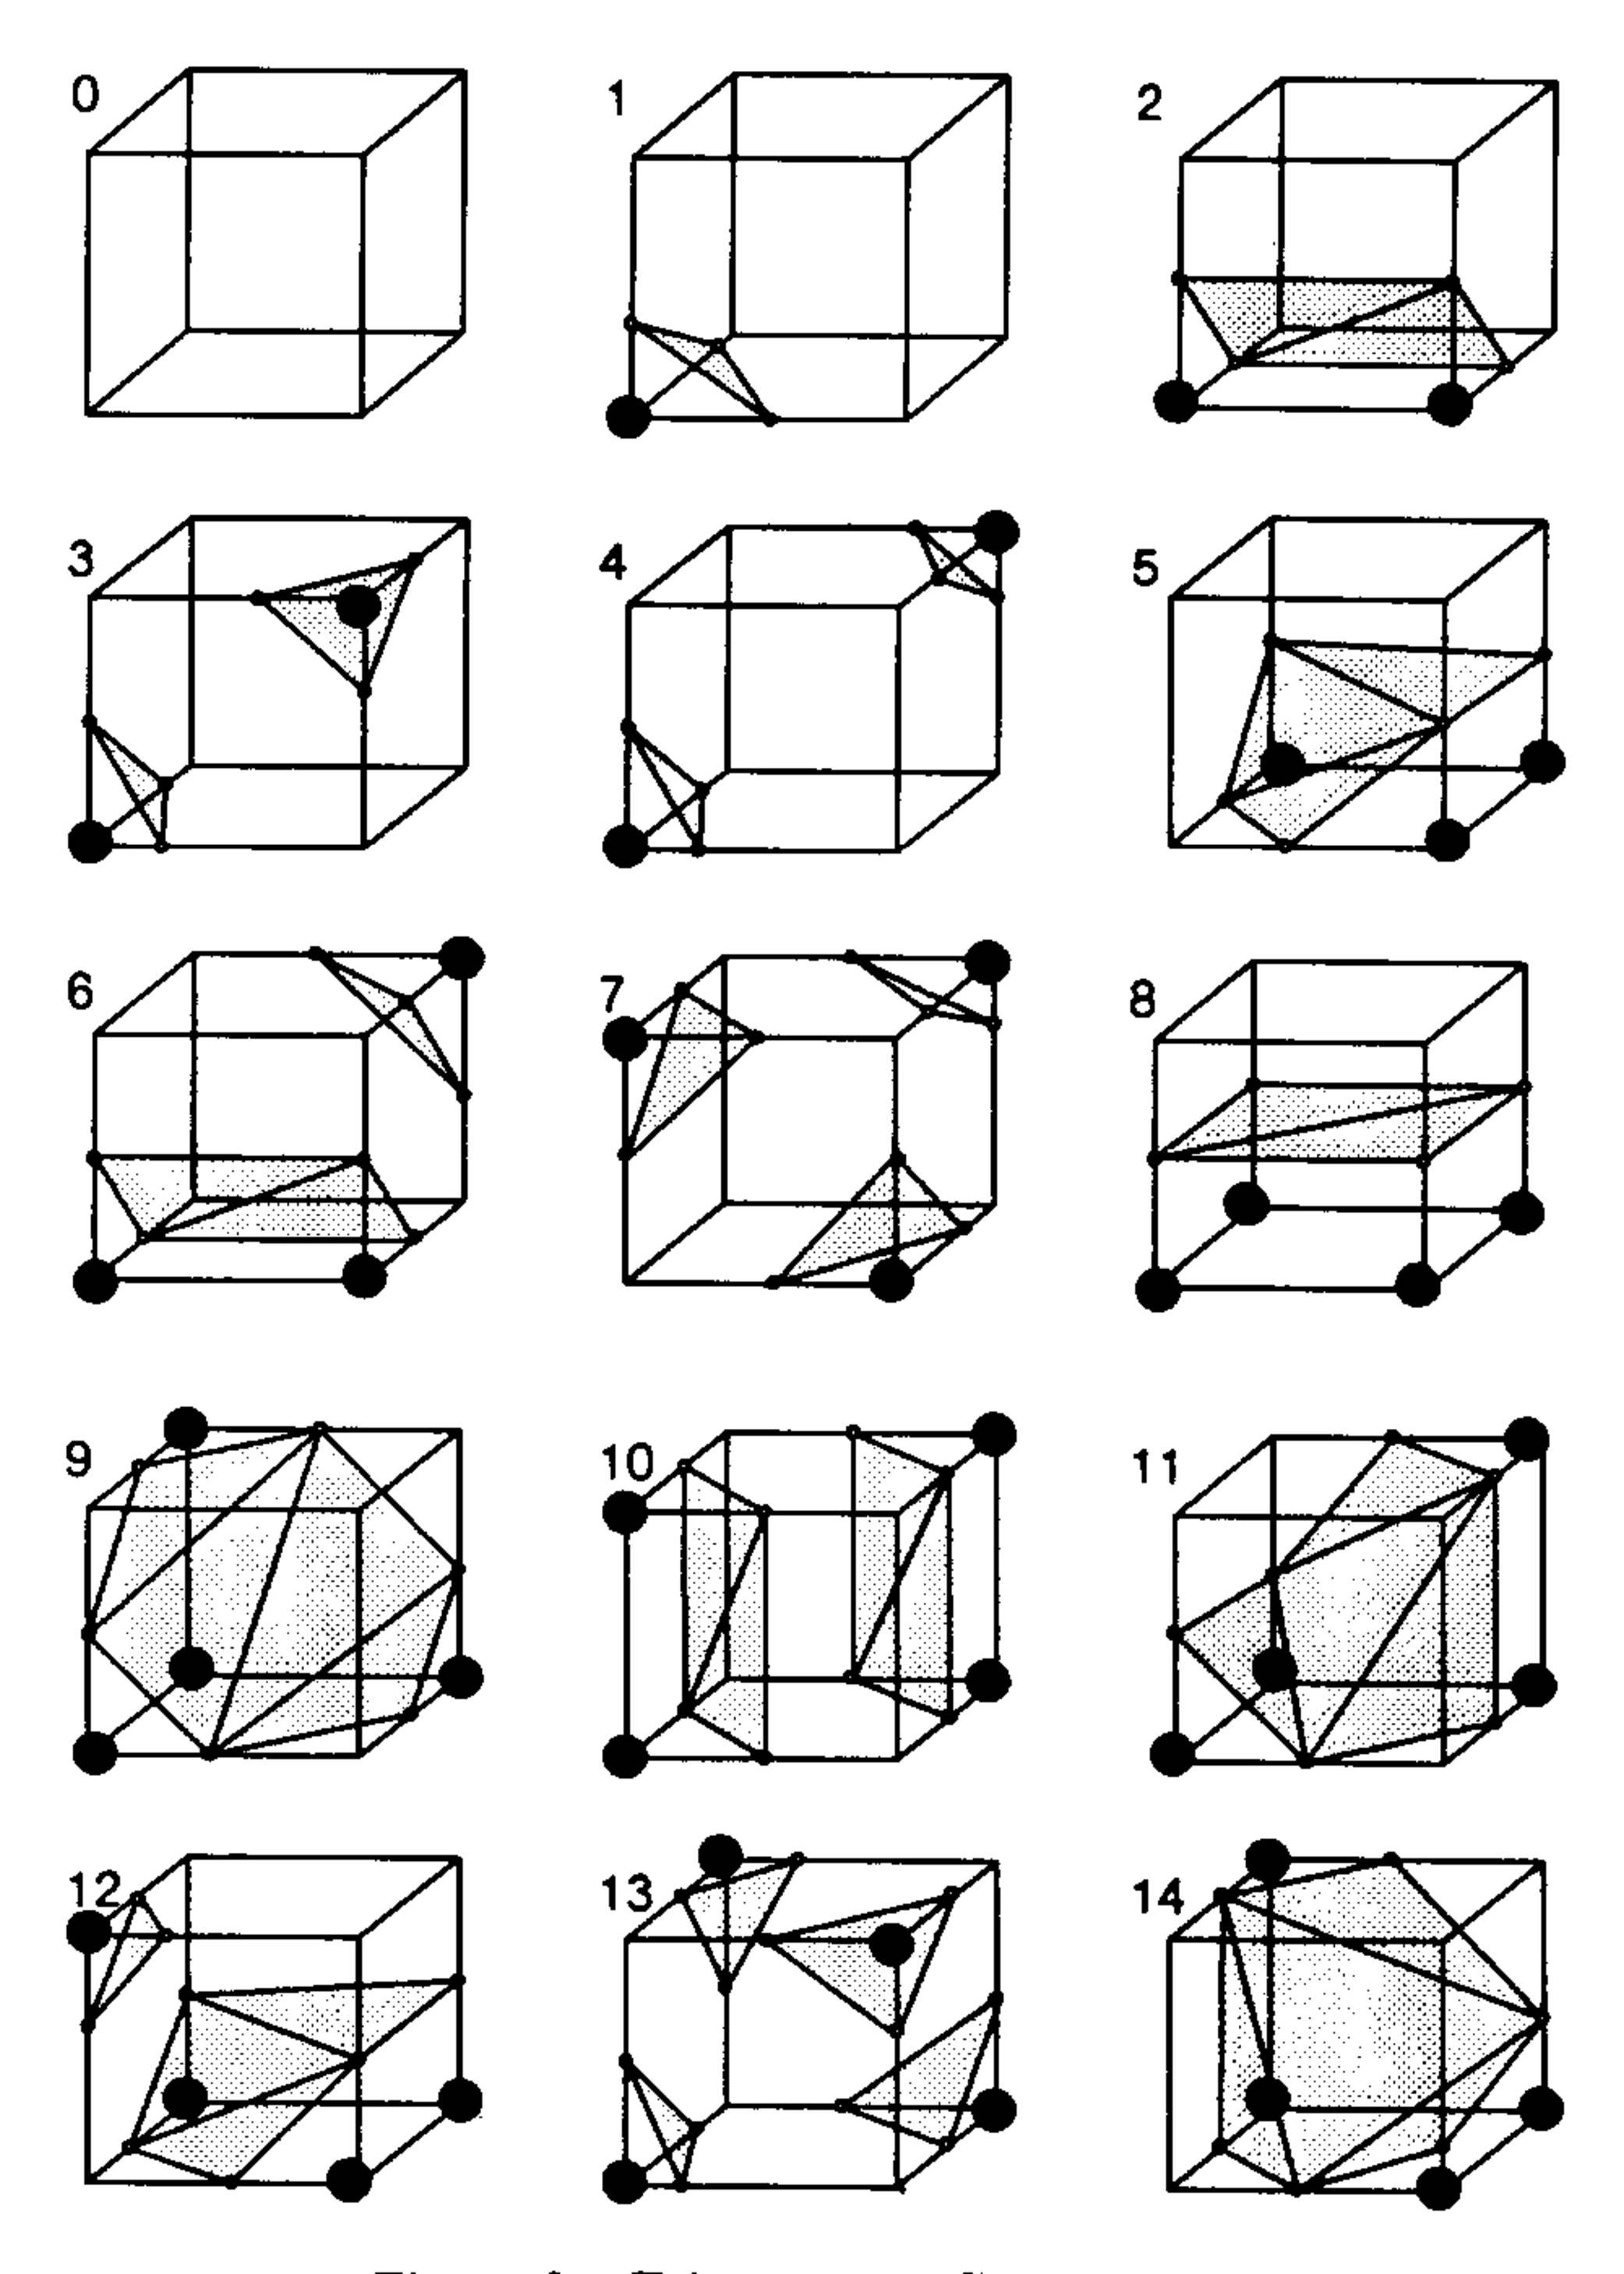
\includegraphics[width=0.6\textwidth]{Images/MCTable.pdf}
  \caption{Unique triangulations of the cubes according to Lorensen and
  Cline. Image from the original Marching Cubes publication~\cite{MC}.}
  \label{fig:MCTable}
\end{figure}

%%%%%%%%%%%%%%%%%%%%%%%%%%%%%%%%%%%%%%%%%%%%%%%%%%%%%%%%%%%%%%%%%%%%%%%%
\section{The Parallel Vectors Operator}\label{sec:PVO}
%%%%%%%%%%%%%%%%%%%%%%%%%%%%%%%%%%%%%%%%%%%%%%%%%%%%%%%%%%%%%%%%%%%%%%%%

When extracting ridge lines in three dimensions, one could check for the
conditions of Equation~\ref{eq:ridgeDot} and~\ref{eq:ridgeEV}. This
would require to extract two isolines simultaneously which is not
possible with the classical Marching Cubes algorithm. Another way would
be to check if the gradient $g$ is parallel to itself derived with the
Hessian, $g || H g$, as this implies that the gradient only changes
along its direction. Peikert and Roth proposed the Parallel Vectors
Operator~\cite{PV} as a versatile tool to find the set of points where
two vector fields are parallel. We will use their analytic solution for
triangular faces, and therefore every face of a cell is split into two
triangles. The vectors of the gradient field and their derivatives at
the nodes of an examined triangle can be expressed as a function of
local triangle coordinates $s$, $t$ and $u$ with $u$ set to $1$:
\begin{equation}
  g = V
  \begin{pmatrix}
    s\\
    t\\
    1
  \end{pmatrix}
\end{equation}
\begin{equation}
  H g = W
  \begin{pmatrix}
    s\\
    t\\
    1
  \end{pmatrix}.
\end{equation}
\noindent $V$ and $W$ are $3 \times 3$ matrices that are constructed
from the vectors $v_i$ and $w_i$ at the three nodes of the fields with:
\begin{align}
  &v_{12} = v_2 - v_1\\
  &v_{13} = v_3 - v_1\\
  &V = (v_1, v_{12}, v_{13})
\end{align}
\noindent and respectively for $w_i$ and $W$. Now two fields are
parallel when:

\begin{equation}
  V
  \begin{pmatrix}
    s\\
    t\\
    1
  \end{pmatrix}
  = \bar{\lambda} W
  \begin{pmatrix}
    s\\
    t\\
    1
  \end{pmatrix}
\end{equation}

\noindent If either $V$ or $W$ is invertible, ergo $\det{(V)}\neq 0 \vee
\det{(W)}\neq 0$ we can adjust the equation to get an eigenvector
problem:

\begin{equation}
  W^{-1} V
  \begin{pmatrix}
    s\\
    t\\
    1
  \end{pmatrix}
  = \bar{\lambda}
  \begin{pmatrix}
    s\\
    t\\
    1
  \end{pmatrix}
\end{equation}

\noindent Usually the matrix with the larger determinant is being
inverted. Now we can calculate the eigenvectors for the matrix $W^{-1}
V$ and scale them such that their last component is $1$. This provides
us with the local triangle coordinates $s$ and $t$ where the two fields
are parallel. If $s+t \leq 1$ and $s$ and $t$ are both greather than
zero, the point lies within the triangle and an extremum is found. With
the triangle coordinates the Hessian at the point can be interpolated to
check for $\lambda_2 < 0$ in the case of ridges or $\lambda_2 > 0$ for
valleys. Alternatively the minor or major eigenvectors of the Hessian
can be tested for parallelity, depending on the desired feature.

  %%%%%%%%%%%%%%%%%%%%%%%%%%%%%%%%%%%%%%%%%%%%%%%%%%%%%%%%%%%%%%%%%%%%%%%%
\chapter{Method}\label{chap:Method}
%%%%%%%%%%%%%%%%%%%%%%%%%%%%%%%%%%%%%%%%%%%%%%%%%%%%%%%%%%%%%%%%%%%%%%%%

This chapter explains our principle approach on how to extract ridge
features from uncertain scalar fields. In the usual case, ridges do not
lie directly on the nodes of a cell, but inbetween. Therefore it is
insufficient to only look at single nodes of every member of the set of
possibly correlated scalar fields to decide on the presence of a ridge.
Thus in the $3$-dimensional case the actual node at the location we
examine is the bottom left node of a cell of 8 nodes (see red node in
Figure~\ref{fig:3DNH}). This follows an implementation detail, as the
scalar fields in our case are traversed from bottom left to top right.
Sampling these 8 nodes with a Monte-Carlo method would only give us
Gaussian distributed values over the range of values at these locations,
but no information about their change in either dimension outside the
cell. Otto and Theisel~\cite{Vortex} tested in their work to derive a
velocity vector $v$ in a two dimensional uncertain vector field by
sampling the vector and its four neighboring vectors individually from
their distributions. They then estimated the Jacobian $J$ with central
differences on the neighboring vectors and multiplied it with the
velocity vector, to get the acceleration vector $a = J v$. The resulting
vectors were not Gaussian distributed anymore. They solved this issue by
instead of sampling each vector individually, they sample the whole
neighborhood of the vector to keep track of its change along the
dimensions. Therefore we also inspect the 24 nodes adjacent to the 8
nodes of the cell, to be able to calculate the gradient via central
differences. As Theisel \etal{} were searching for vortex core lines in
uncertain vector fields, they only needed to derive their field once, to
be able to decide on the presence of a core line based on the
eigenspace. As we base our detections on eigenvalues and vectors as
well, we need to derive our uncertain scalar field twice. We therefore
also add the adjacent nodes of the 24 supporting nodes to our considered
neighborhood. This leads to 80 nodes making up the cell we want to draw
samples from (see Figure~\ref{fig:NH}). With this we can create the
uncertain scalar field from Section~\ref{sec:USF}.

%%%%%%%%%%%%%%%%%%%%%%%%%%%%%%%%%%%%%%%%%%%%%%%%%%%%%%%%%%%%%%%%%%%%%%%%
\section{Multivariate Gaussian Sampling}\label{sec:MGS}
%%%%%%%%%%%%%%%%%%%%%%%%%%%%%%%%%%%%%%%%%%%%%%%%%%%%%%%%%%%%%%%%%%%%%%%%

Our uncertain scalar field $S_{\mathcal{N}}$ at point
$x=(x_1,\dots,x_n)$ consists of a multivariate Gaussian distribution,
made up from the mean vector $\mu_x$ and the covariance matrix $\Sigma_x$. The
mean vector portrays the average values of the neighborhood of $x$ while
the covariance matrix contains the variances of each value to each other
around this mean. Unfortunately we cannot compute ridge criteria from
these objects. Monte-Carlo methods offer a way to draw samples from
multivariate normal distributions. The basis of this method is the affine
transformation property of normal distributed vectors that states that
any linear transformation of a normal vector is again normal:

\begin{equation}
    X \sim \mathcal{N}(\mu,\Sigma) \Rightarrow AX \sim \mathcal{N}(A\mu, A\Sigma A)
\end{equation}

\noindent for any dimensionality $d$ of vector $X$ and $d \times d$
matrix $\Sigma$ and any $k \times d$ matrix $A$. By this property we
know that if we have a standard normal distributed vector $Z \sim
\mathcal{N}(0,I)$ with $I$ being an $d \times d$ identity matrix, then
$X = AZ + \mu$ is from the distribution $X \sim \mathcal{N}(\mu, A
A^\top)$. Now we simply have to find a matrix $A$ for which $AA^\top =
\Sigma$. The Cholesky (Section~\ref{sec:cholesky}) and the
Eigendecomposition (Section~\ref{sec:eigen}) are the two most popular
methods to calculate such a matrix as the Cholesky decomposition is
computationally efficient and the Eigendecomposition deliveres more
numerical stability as well as a lot of predefined librarys. As our
covariance matrices are only positive semi-definite, we need the
extended version of Cholesky. Now we get the two decompositions:
\begin{align}
    &\Sigma_x = L D L^\top \\
    &\Sigma_x = E \Lambda E^{-1},
\end{align}
In theory, a suitable matrix $A$ would now be either $A=L
D^{\frac{1}{2}}$ or $A=E\Lambda^{\frac{1}{2}}$ for $\Sigma = AA^\top$.
In practice, because of our relatively huge $80 \times 80$ dimensional
covariance matrix we get negative elements in the diagonal matrix $D$
even though our covariance matrix is positive semi-definite. Therefore
we cannot take the root of $D$. The same issue goes for the
Eigendecomposition where the eigenvalues become infinitesimally small
negative values, hindering the computation of the root of $\Lambda$. As
the sign of the eigenvalues determines the definiteness of a matrix,
this makes our covariance matrix technically indefinite, as we have
positive and negative eigenvalues. We solved this issue by simply
multiplying the components without taking the root of the diagonal
matrix, hence $A = LD$ and $A = E \Lambda$. This did not seem to affect
the samples drawn with the Eigendecomposition, but the samples drawn
with Cholesky showed some inconsistencies. Section (INSERT REF) will
give more insight on that topic and compare the decompositions. Now we
can proceed with the found $A$. In the 3 (2) dimensional  case we
generate an 80 (24) dimensional standard uniformly distributed vector
and transform it into a standard normal distributed vector $Z$ using
the Box-Muller transformation (Section~\ref{sec:BM}). Now we multiply
$A$ with $Z$ and add the mean vector of this location to get the sample
vector $X = AZ + \mu_x, X \sim \mathcal{N}(\mu_x, \Sigma_x)$. This is
only a single instance from the multivariate distribution, thus we
repeat the sampling multiple times per cell to try to model the
distribution as best as possible. With the now obtained sample vectors
we can start to calculate ridge criteria at the location.

%%%%%%%%%%%%%%%%%%%%%%%%%%%%%%%%%%%%%%%%%%%%%%%%%%%%%%%%%%%%%%%%%%%%%%%%
\section{Processing the cell}\label{sec:proc}
%%%%%%%%%%%%%%%%%%%%%%%%%%%%%%%%%%%%%%%%%%%%%%%%%%%%%%%%%%%%%%%%%%%%%%%%

  %%%%%%%%%%%%%%%%%%%%%%%%%%%%%%%%%%%%%%%%%%%%%%%%%%%%%%%%%%%%%%%%%%%%%%%%
\chapter{Evaluation}\label{chap:Eval}
%%%%%%%%%%%%%%%%%%%%%%%%%%%%%%%%%%%%%%%%%%%%%%%%%%%%%%%%%%%%%%%%%%%%%%%%

This chapter will evaluate the results obtained with our new criterion,
compare them with the conventional method, as well as show its vantages
and disadvantages. But at first, we will talk about the differences of
the matrix decompositions used to generate the samples from the
multivariate distributions.

%%%%%%%%%%%%%%%%%%%%%%%%%%%%%%%%%%%%%%%%%%%%%%%%%%%%%%%%%%%%%%%%%%%%%%%%
\section{Comparison of Matrix Decompositions}\label{chap:evalMD}
%%%%%%%%%%%%%%%%%%%%%%%%%%%%%%%%%%%%%%%%%%%%%%%%%%%%%%%%%%%%%%%%%%%%%%%%

Multivariate Gaussian sampling is a common way to model distributions
by drawing variants from the set. This method makes use of the
factorization of the covariance matrix $\Sigma$ from the distribution into
the product of two matrices, such that $\Sigma = AA^\top$. Literature
like ``Random Number Generation and Monte Carlo Methods''~\cite{Monte}
state, that any decomposition that achieves such a factorization is
suitable for the genration of random samples and delivers equally
good results. Therefore one could prefer the Cholesky decomposition
because of its faster computation time $\mathcal{O}(N^3/3)$ over
the Eigendecomposition with $\mathcal{O}(N^3)$. To compare the two
decompositions, we take the function from Figure~\ref{fig:sfield} and
equally shift it along the $x$-dimension to create a set of twenty
members with a high uncertainty along $x$, but no uncertainty along
the other dimensions, ridgewise. Figure~\ref{fig:decomps} shows the
result of the uncertain ridge calculation for both decompositions using
the new criterion. The surfaces exhibit heavy differences. While the
Eigendecomposition deliveres a smooth estimation with a constant high
probability for the ridges that every field contains and a blue cloud
with low probability where the ridge is uncertain, Cholesky has a
distorted ridge perpendicular to $y$ as well as three to four distinct
ridge structures across $x$ with a low probability. The result of the
Cholesky decomposition is considerably worse.

\begin{figure}
    \begin{subfigure}[b]{0.49\textwidth}
        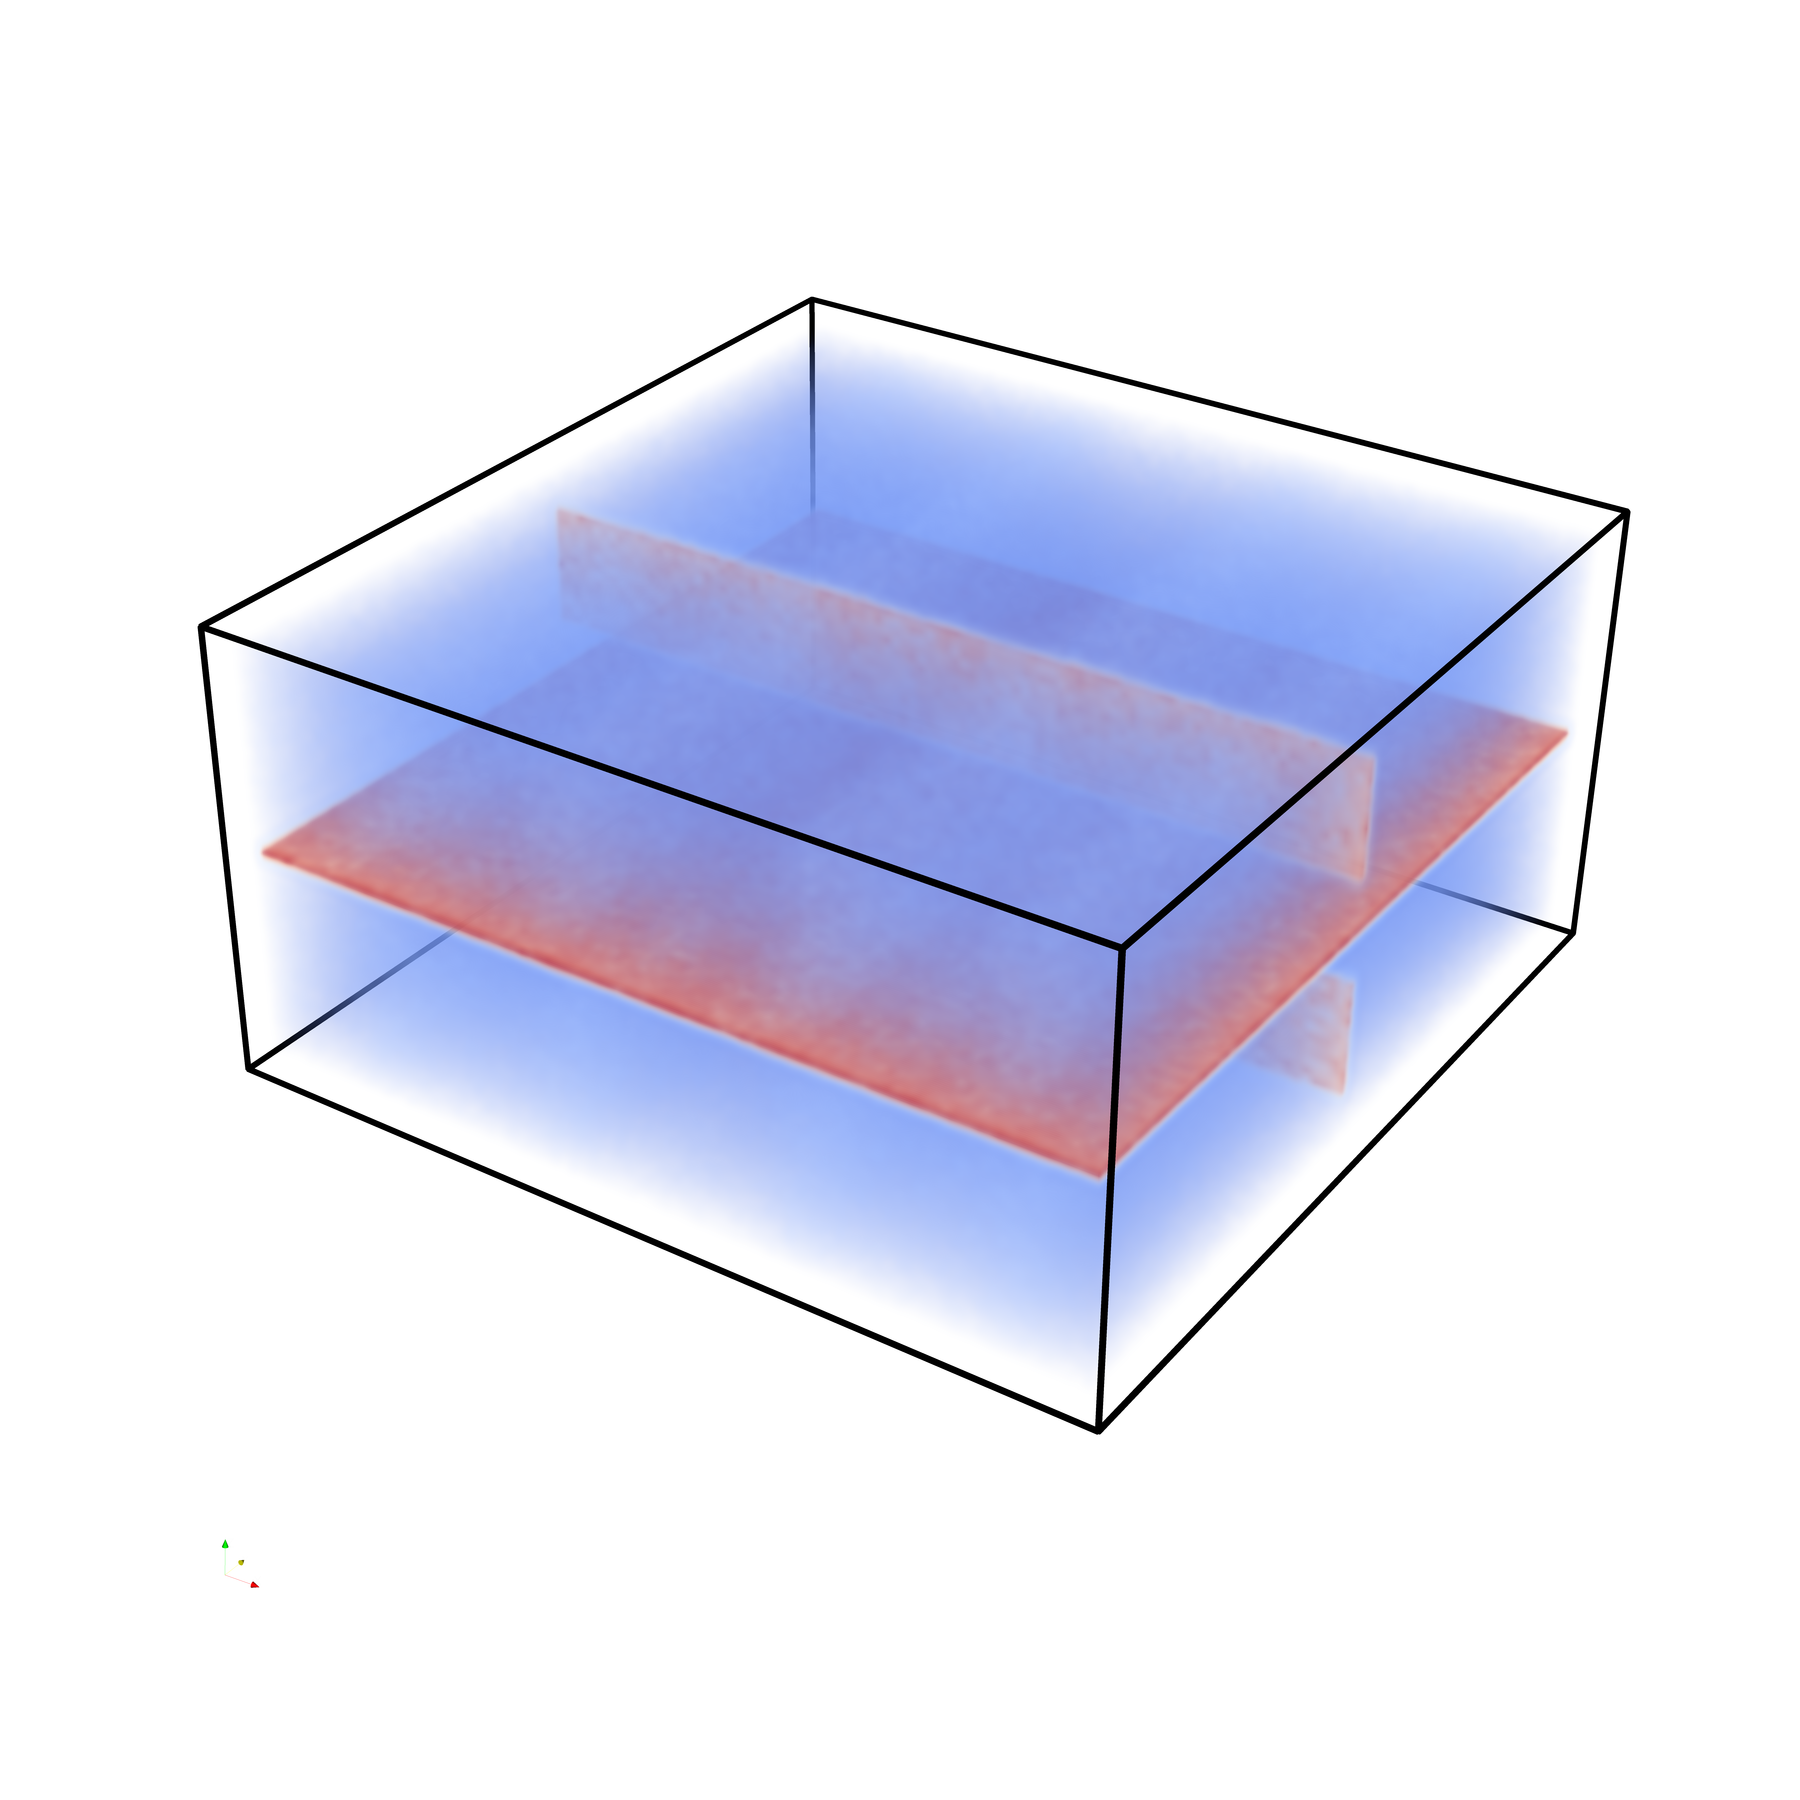
\includegraphics[width=\textwidth]{Images/shiftXeigen.png}
        \caption{Eigendecomposition}
        \label{fig:shiftXeigen}
    \end{subfigure}
    \begin{subfigure}[b]{0.49\textwidth}
        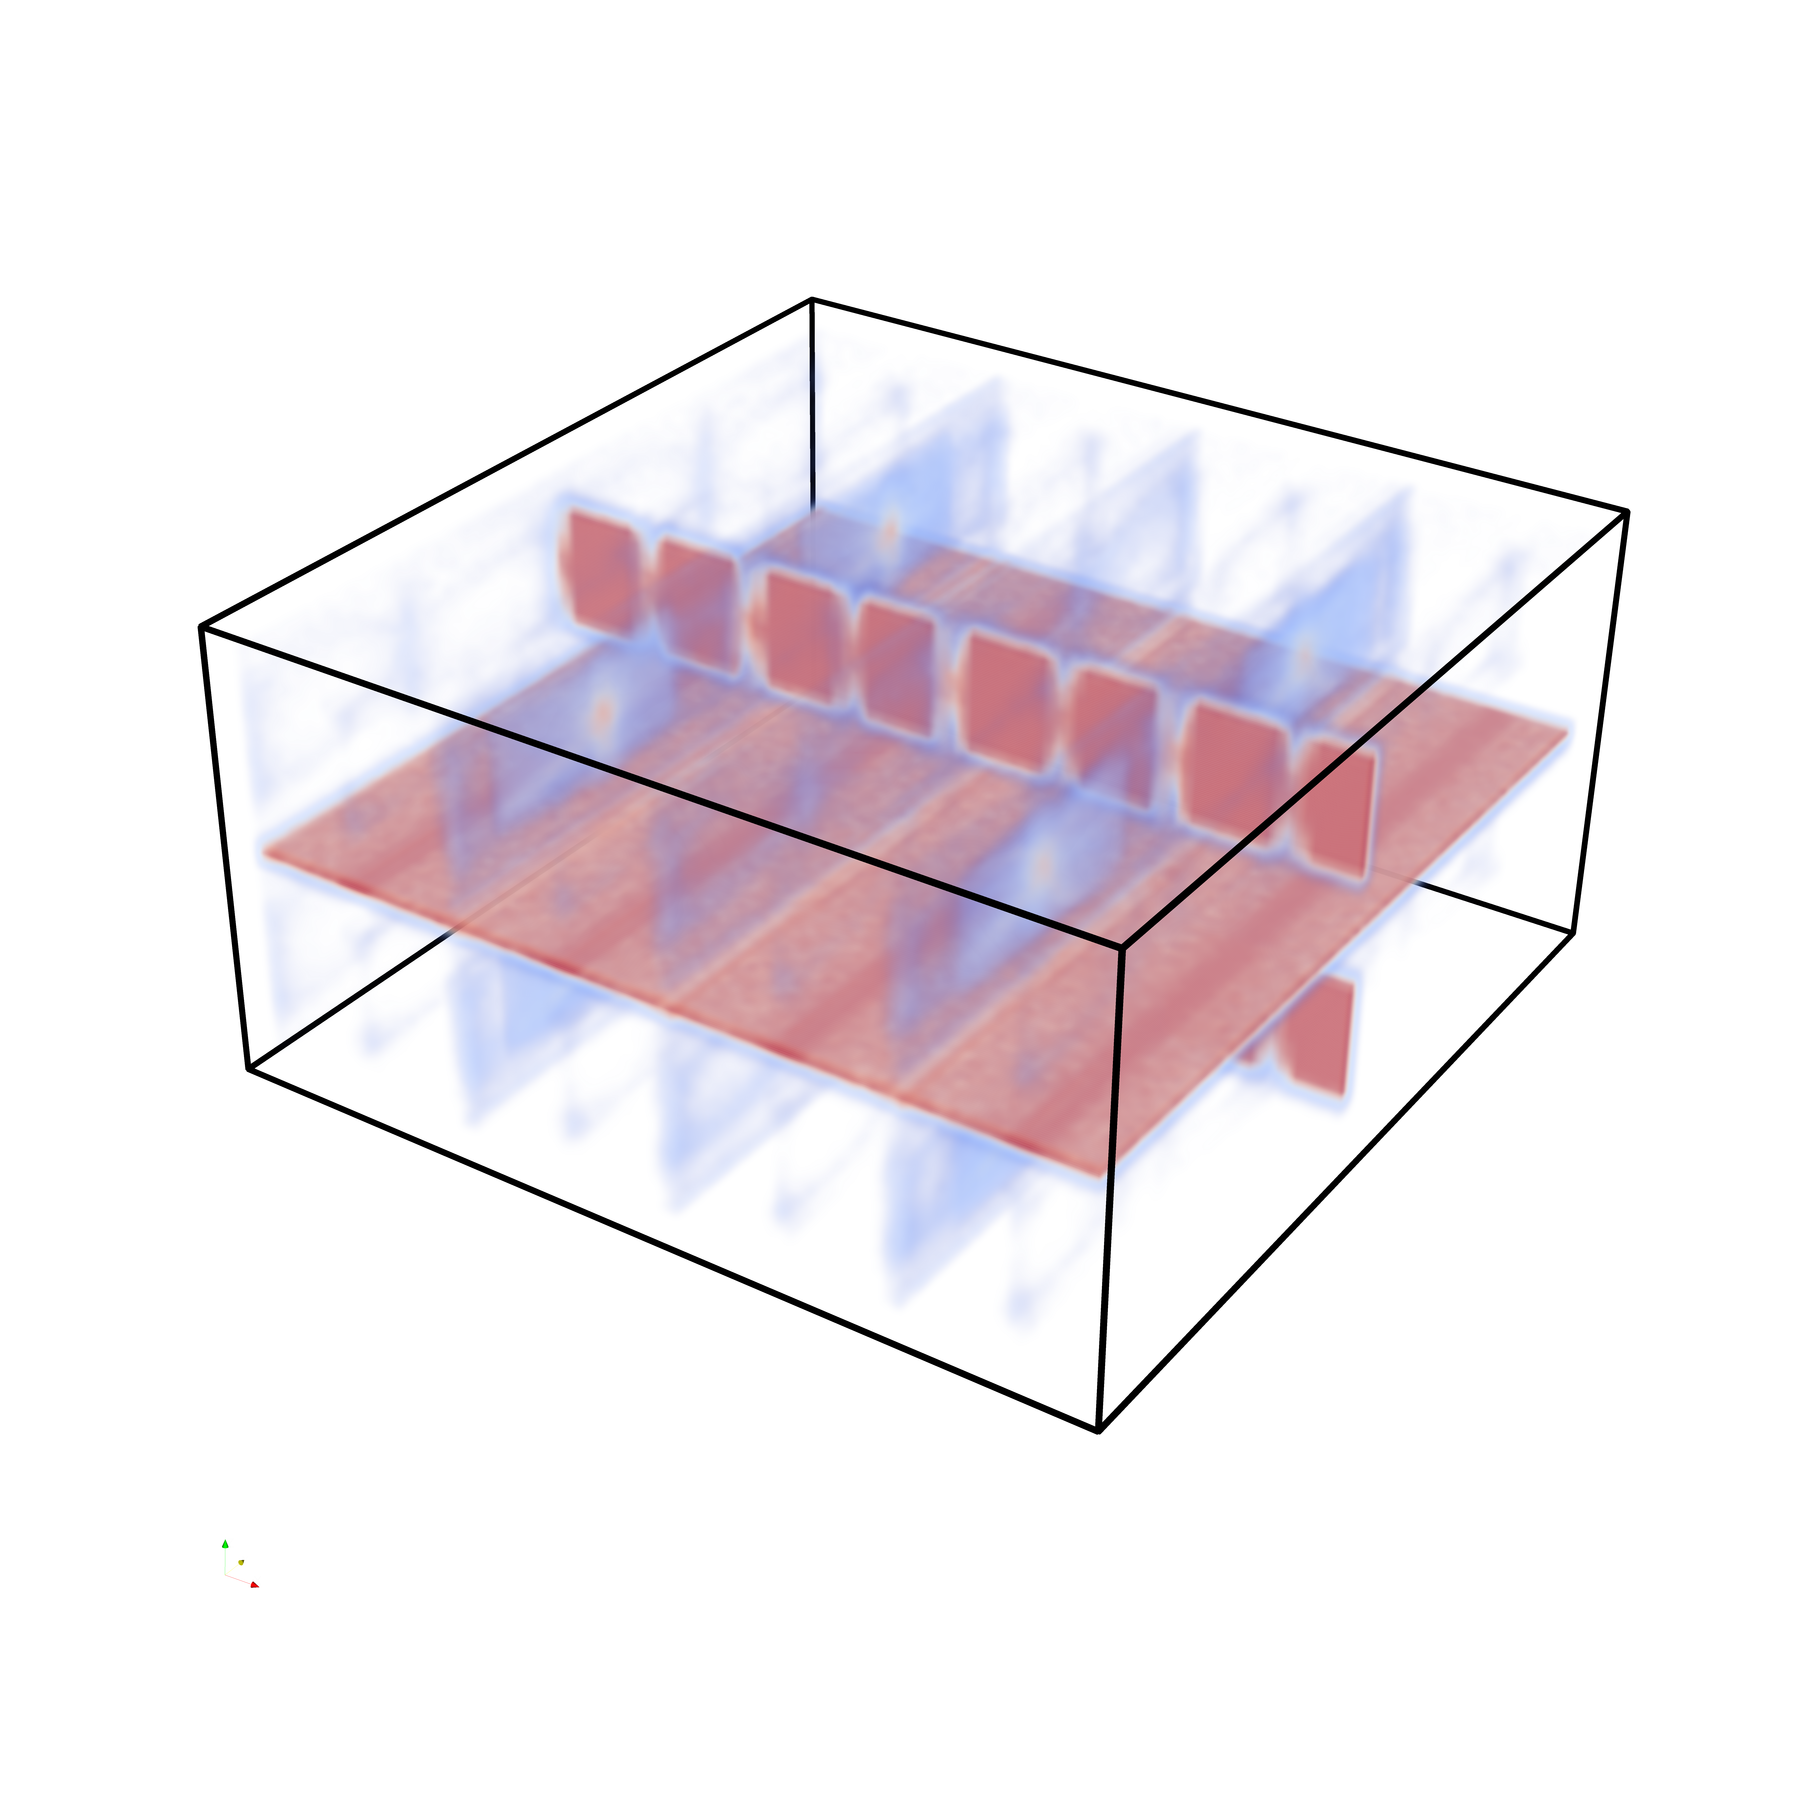
\includegraphics[width=\textwidth]{Images/shiftXcholesky.png}
        \caption{Cholesky}
        \label{fig:shiftXcholesky}
    \end{subfigure}
    \caption{Comparison of the two matrix decompositions for a set
    of fields shifted equally along the $x$ dimension. The 
    Eigendecomposition gives a smooth estimate of the ridge surface,
    according to the distribution of the ridges in the members.
    Cholesky exhibits lower probabilities at points where the
    ridge is very certain.}
    \label{fig:decomps}
\end{figure}

To understand what happened here, we will again take a look at
samples drawn from the distribution of Figure~\ref{fig:sampComp}.
Figure~\ref{fig:MDsampComp} shows the gradients of two samples from
either decomposition with their respective unscaled eigenvectors at the
base. Even though the Eigendecomposition in Figure~\ref{fig:sampleEig}
breaks the parallelity of the original field, the gradients still point
in the same general direction and the eigenvectors are consistently
oriented. The gradients of Cholesky on the other hand have no
directional correlation at all. The direction of the vectors is
arbitrary along the distribution and therefore their eigenvectors
have inconsistent orienting as well. The Eigendecomposition seems
to keep the correlation of elements of individual members, whereas
Cholesky mingles the members in one sample. For the calculation of
a ridge feature which depends on precision, this is an issue. The
differences are the consequence of the immanent nature of the
decompositions. The Eigendecomposition of the covariance matrix
equals to the Principal Component Analysis and therefore the scaled
eigenvectors equal to the uncertainty of $\Sigma$ along
the direction of the eigenvector. If we now multiply a standard normal
distributed vector $N$ with $A = E\Lambda$, every $i$-th component of
$N$ is multiplied with a component of the $i$-th column of $A$, and thus
the $i$-th eigenvector. This leads to a constant scaling of elements
along the direction of the eigenvectors. Cholesky produces a lower
triangular matrix for $A=LD^{\frac{1}{2}}$, thus the columns have
increasing influence on the distribution of the sample with increasing
$i$, but the first element of the sample vector is only determined by
the scaling of $a_{11}$ with the random number at $N_1$. An interesting
implementation detail is, that the algorithm calculating the eigenvalues
for our large covariance matrices uses the power iteration method, that
estimates the largest absolute eigenvalue $\lambda$ in $\mathcal{O}
(N^2)$. Then the matrix is reduced by $A-\lambda I$ and power iteration
is applied again. This process can be repeated until all eigenvalues are
found. Analytic results are too computationally intensive for matrices
of size $80 \times 80$ or $24 \times 24$. Due to this algorithm, the
first column of our eigenvectormatrix always corresponds to the largest
eigenvalue, and therefore the axis with the greatest variance of the
set. Comparing this to the Cholesky decomposition, we could say that the
samples from Cholesky are mainly influenced by one axis of variance of
the data set, and decreasingly influenced by the latter variances,
resulting in more random samples. Ond\v{r}ej Straka \etal{\cite{MD}}
studied the different matrix decompositions in the context of Unscented
Kalman Filters, but their results are applicable for our case as well.
They drew three conclusions after their analysis of the decompositions:
If the variable we want to sample contains no correlated elements, the
samples for both decompositions are equally good and therefore the
Cholesky decomposition might be prefered because of its faster
computation time. If the variable contains correlated elements, the
choice may significantly affect the quality of the sample and if the
elements exhibit strong correlation, numerical stability becomes an
issue as well, especially for Cholesky. Considering, that we usually
apply the uncertain ridge extraction to data sets obtained from
simulations, we will have strong correlation of the members of the data
set for the most parts of the field. We will talk about the numerical
stability in Chapter~\ref{chap:Discu}. The difference of the
decompositions is particularly visible when comparing the results
obtained from the ridge extraction using Marching Cubes
(Figure~\ref{fig:MCcomp}). Cholesky produces the same structure as in
Figure~\ref{fig:shiftXcholesky}, but with more certainty. This is a
misleading representation of the underlying uncertainty. The results
obtained from the Eigendecomposition (Figure~\ref{fig:MCeigen}) on the
other hand can almost be considered better than the ones with our new
criterion, as the high probabilities are notably thinner distributed,
just like the certain ridge would be. We will compare the two approaches
in the next section. Concluding from all of this, the Eigendecomposition
delivers better results in most cases. Only if we have strong uncertainty
in the data, the Cholesky decomposition may give us better results.
We took the set from Figure~\ref{fig:MCridges} and extended it with
members having greater variance along either axis. The results of the
two decompositions can be seen in Figure~\ref{fig:HUCcomp}. Here
Cholesky gives us higher probabilities for nodes close to the mean of
the ridges. Due to the high variance of the data set, the members seem
to lose their correlation. The downside is, that this case is not the
usual thing for real world data, where we try to extract ridge structures
from similar scalar fields. 

\begin{figure}
    \begin{subfigure}[b]{0.49\textwidth}
        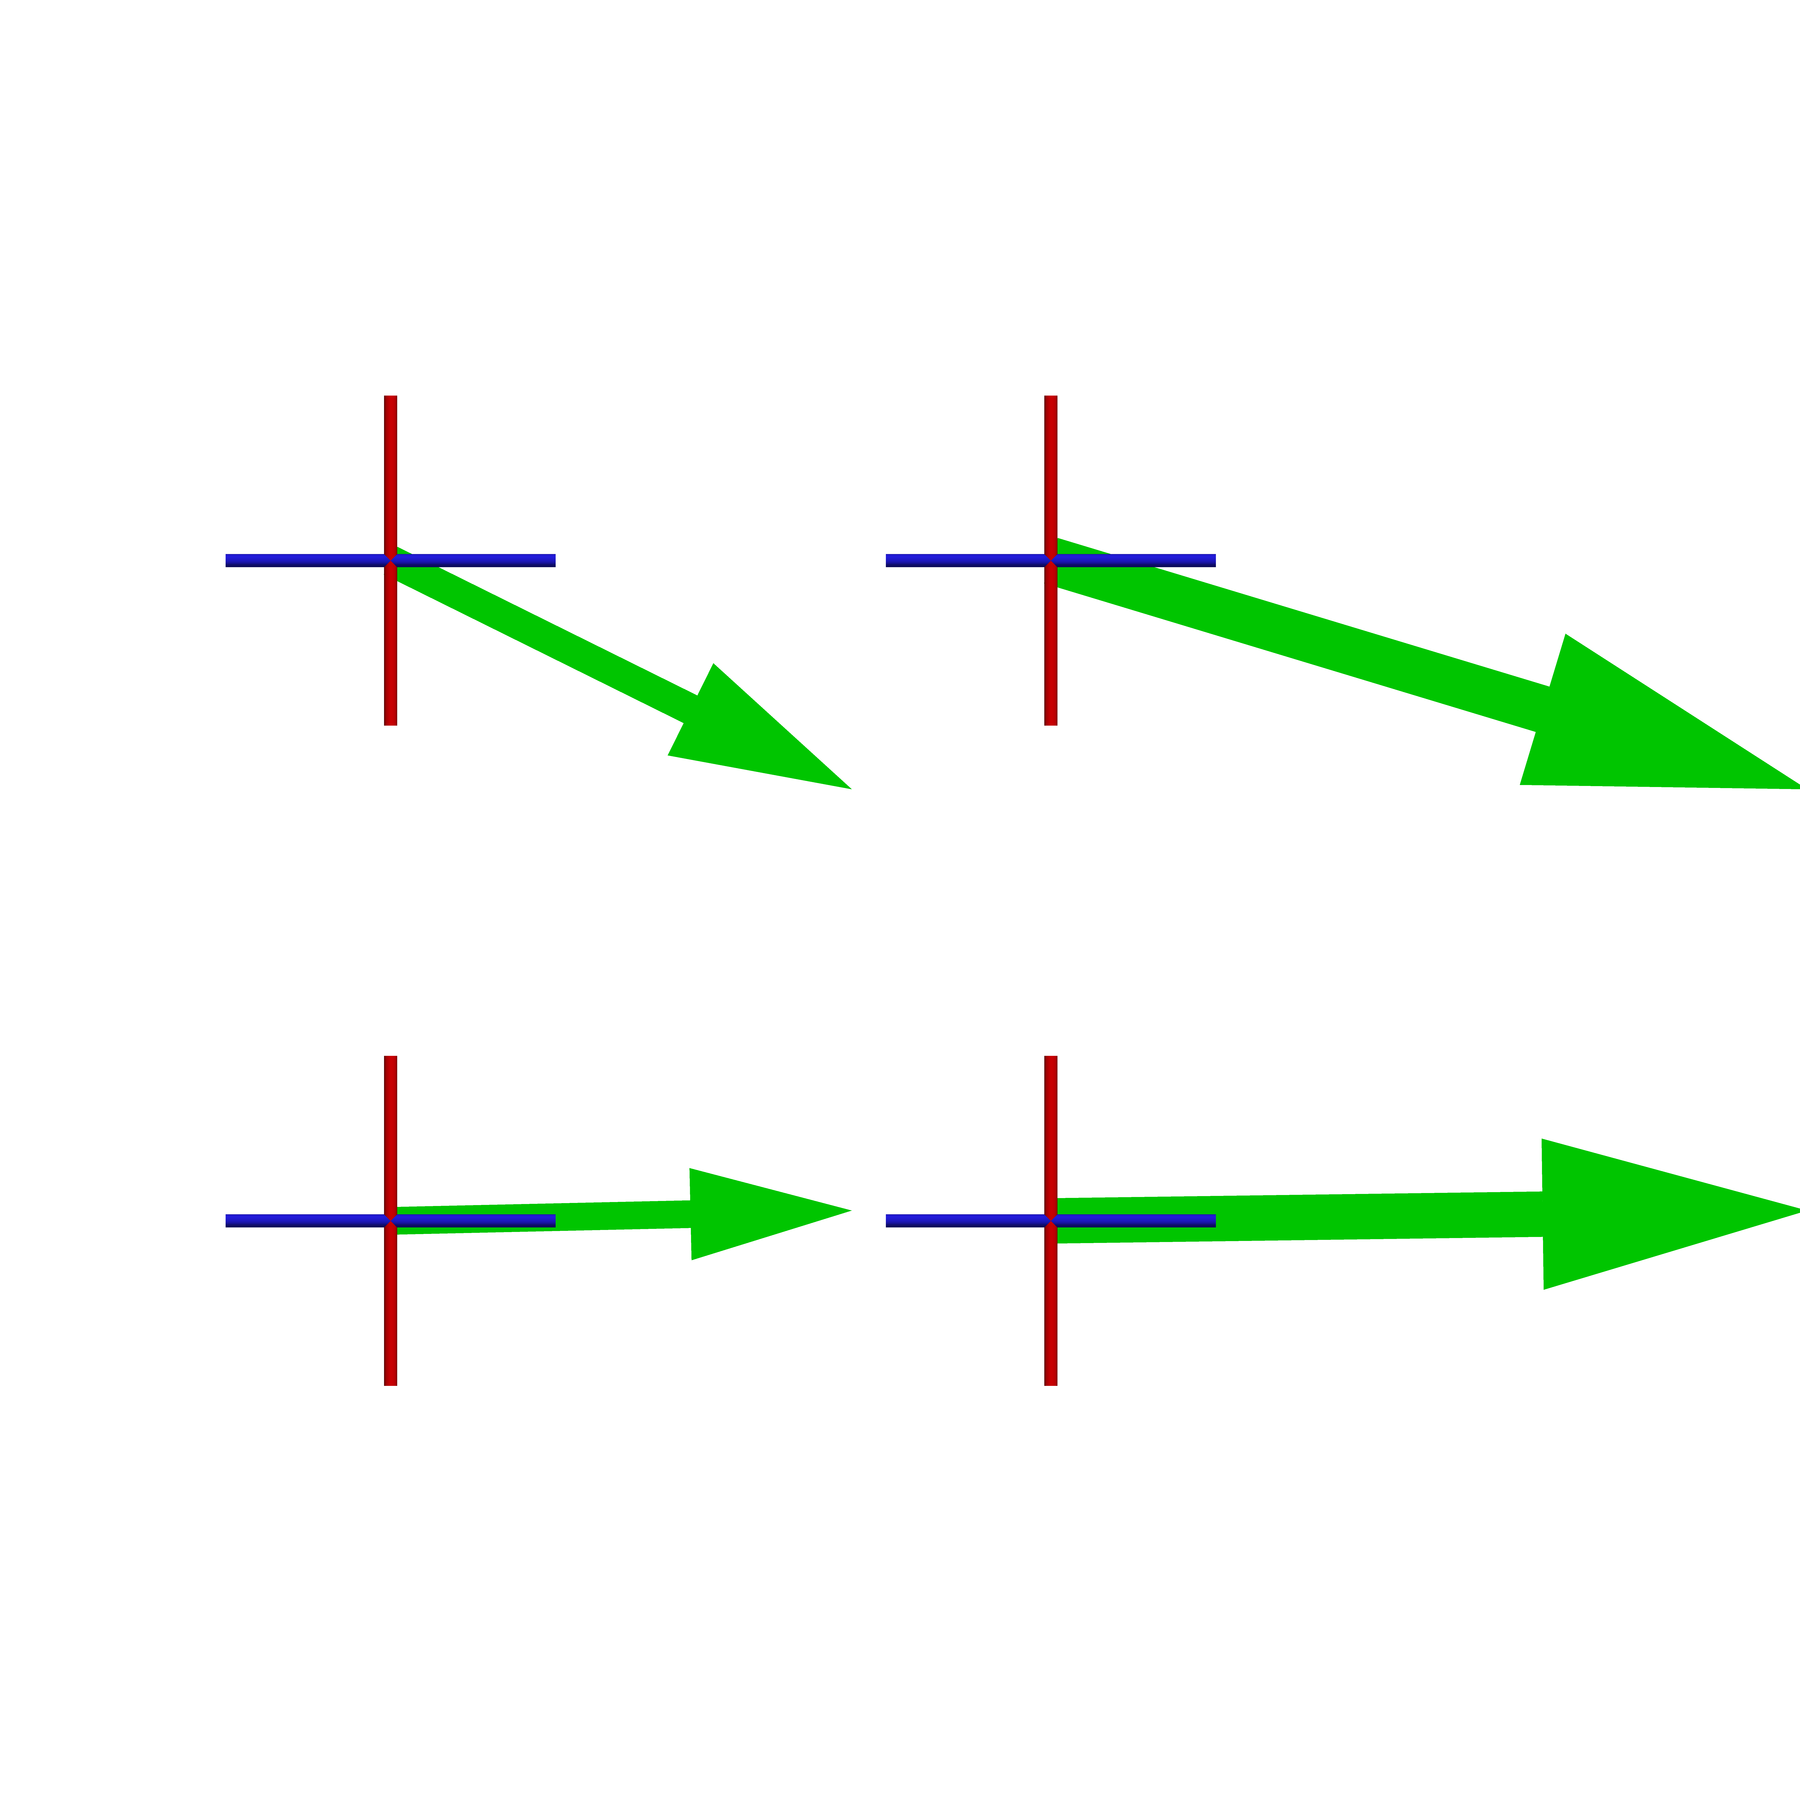
\includegraphics[width=\textwidth]{Images/sampleEig.png}
        \caption{Eigendecomposition}
        \label{fig:sampleEig}
    \end{subfigure}
    \centering
    \begin{subfigure}[b]{0.49\textwidth}
        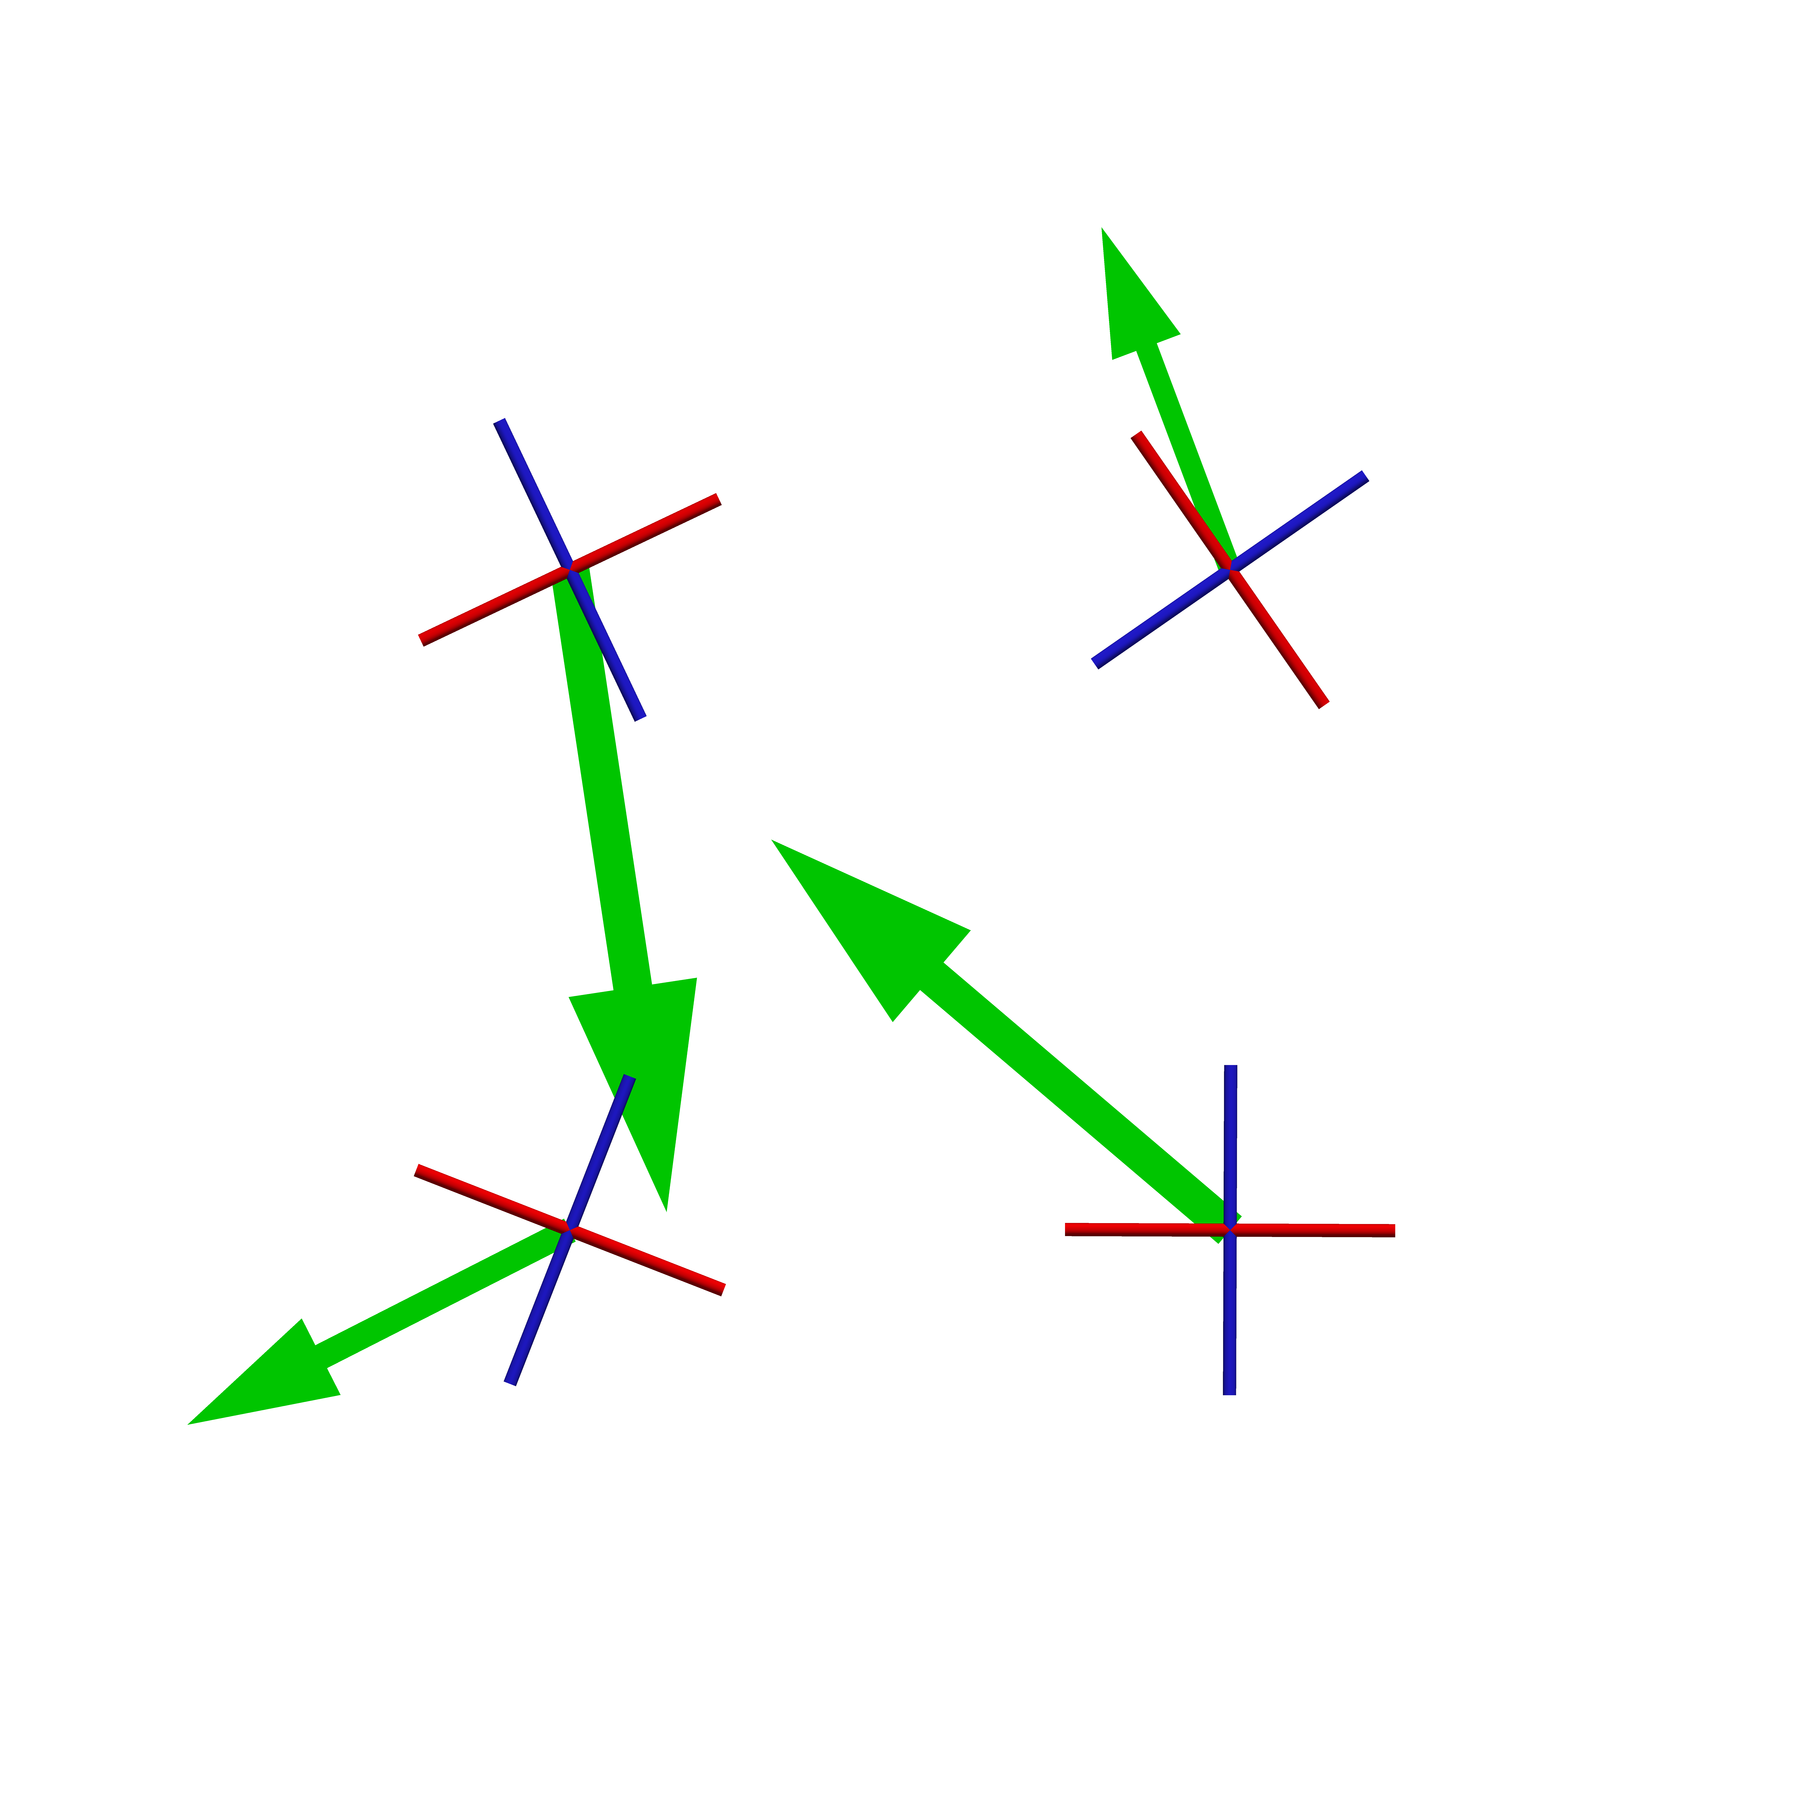
\includegraphics[width=\textwidth]{Images/sampleChol.png}
        \caption{Cholesky}
        \label{fig:sampleChol}
    \end{subfigure}
    \caption{Gradients of samples from the distribution of the rotated
    field for $f(x,y)=x^2$. The samples from the Eigendecomposition
    keep the structure of the original fields, whereas the Cholesky
    decomposition mixes the distributions in one sample.}
    \label{fig:MDsampComp}
\end{figure}

\begin{figure}
    \begin{subfigure}[b]{0.49\textwidth}
        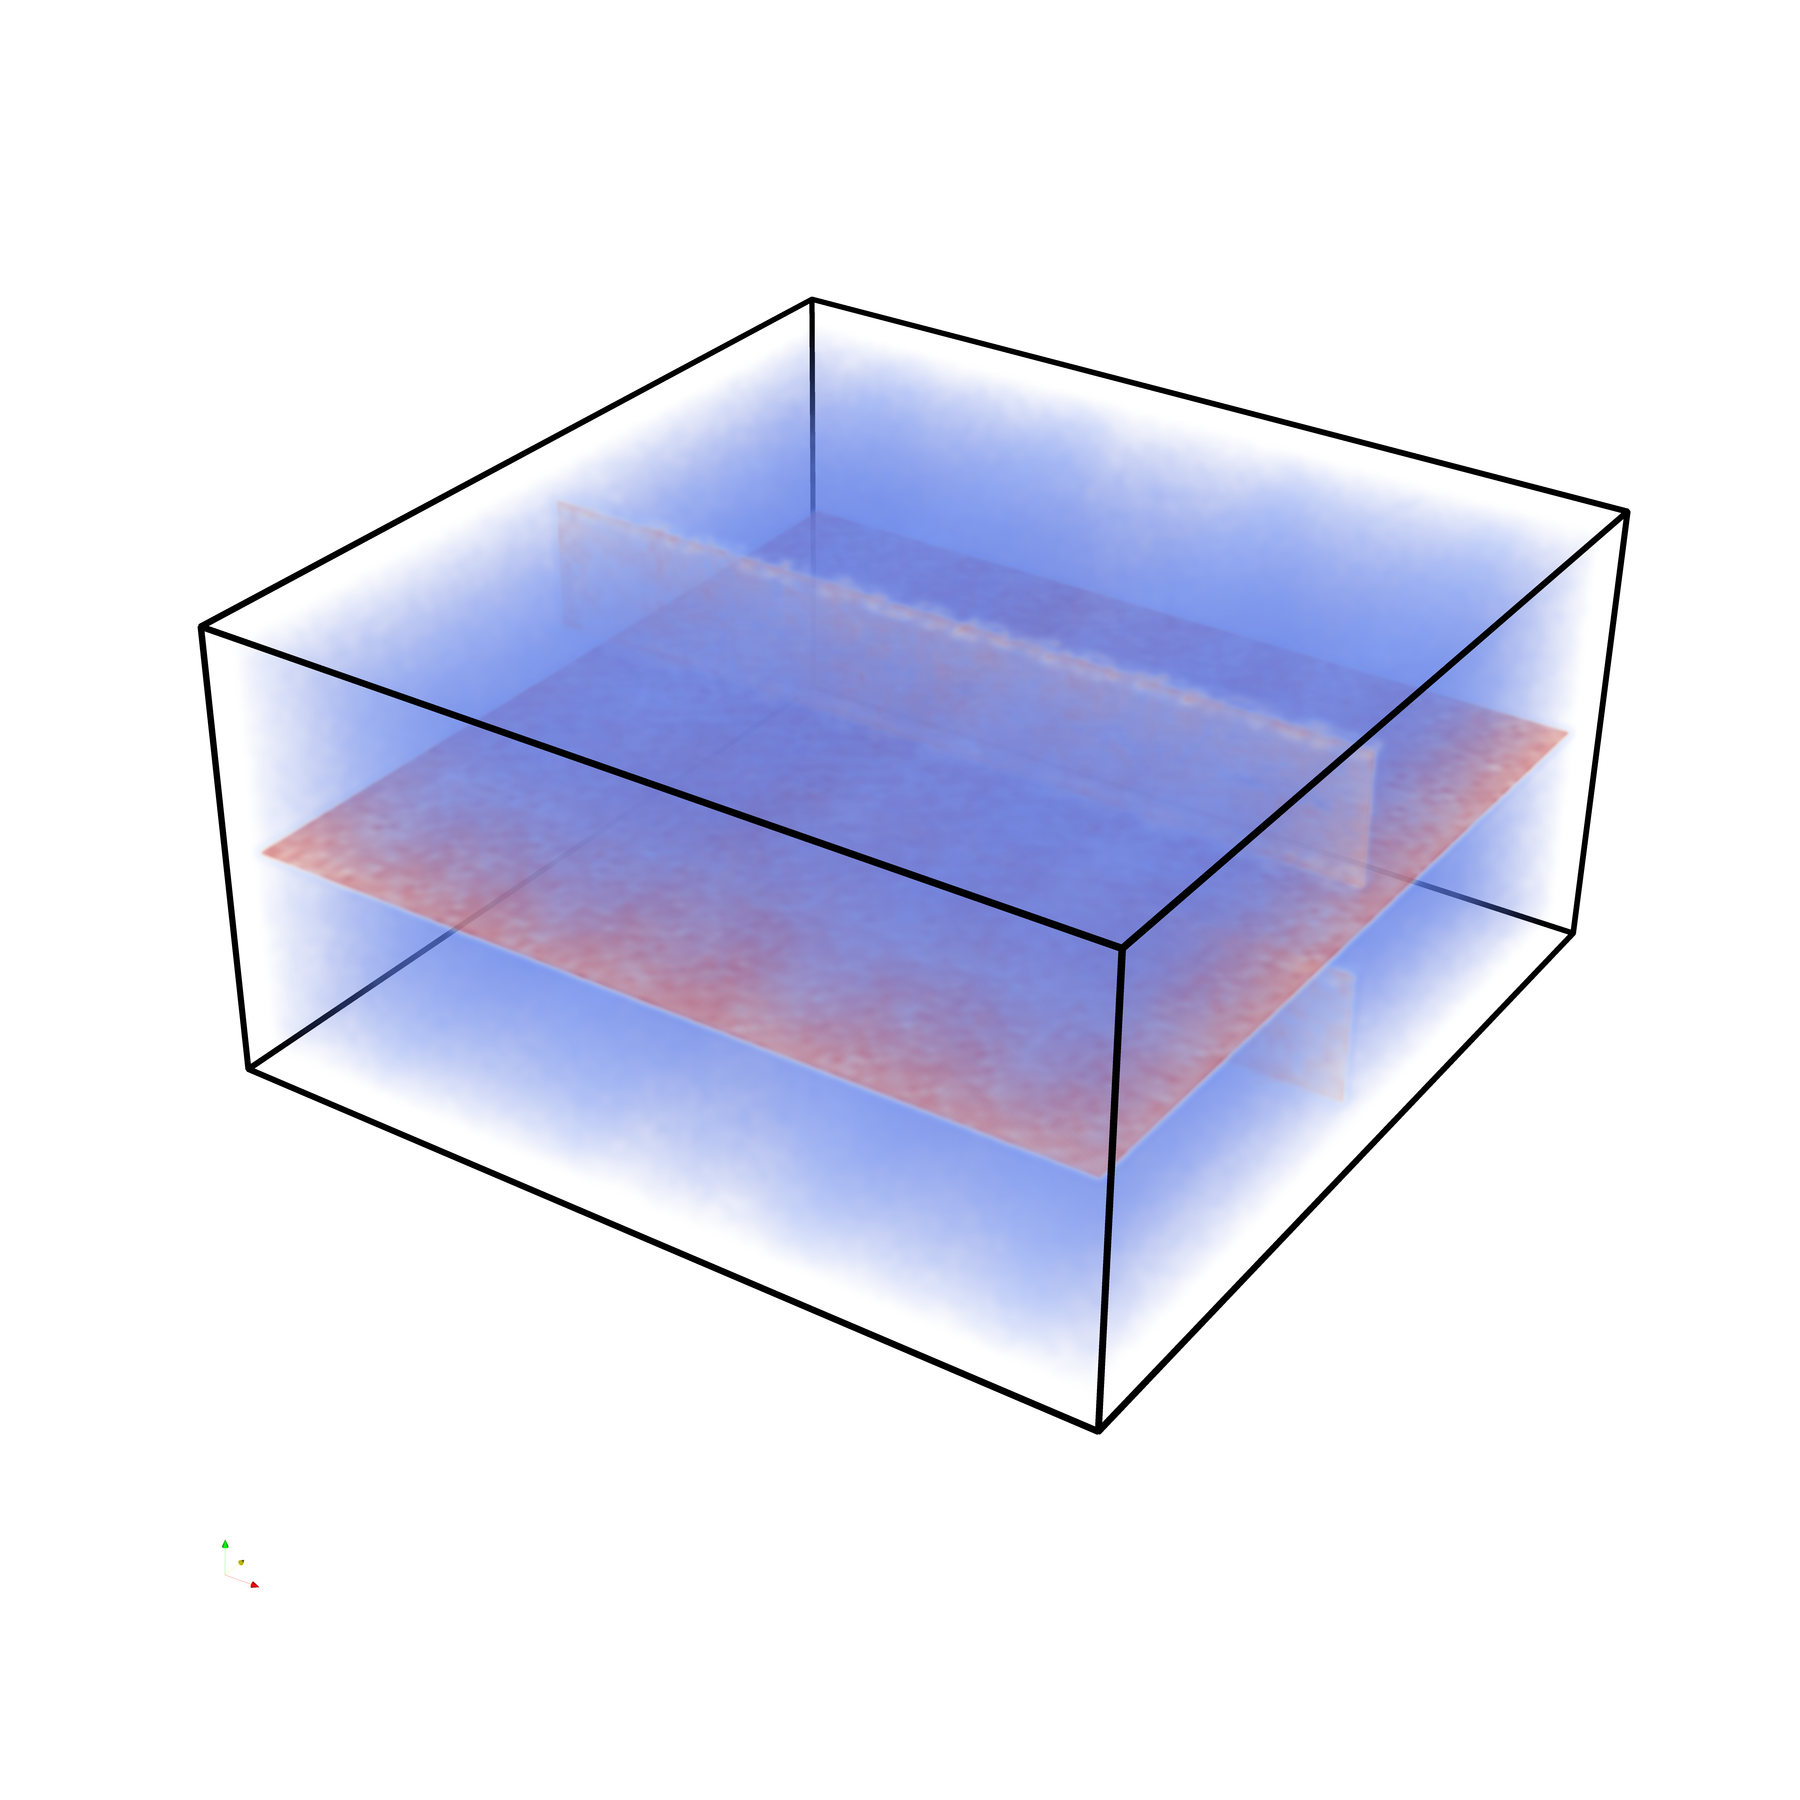
\includegraphics[width=\textwidth]{Images/shiftXold.png}
        \caption{Eigendecomposition}
        \label{fig:MCeigen}
    \end{subfigure}
    \begin{subfigure}[b]{0.49\textwidth}
        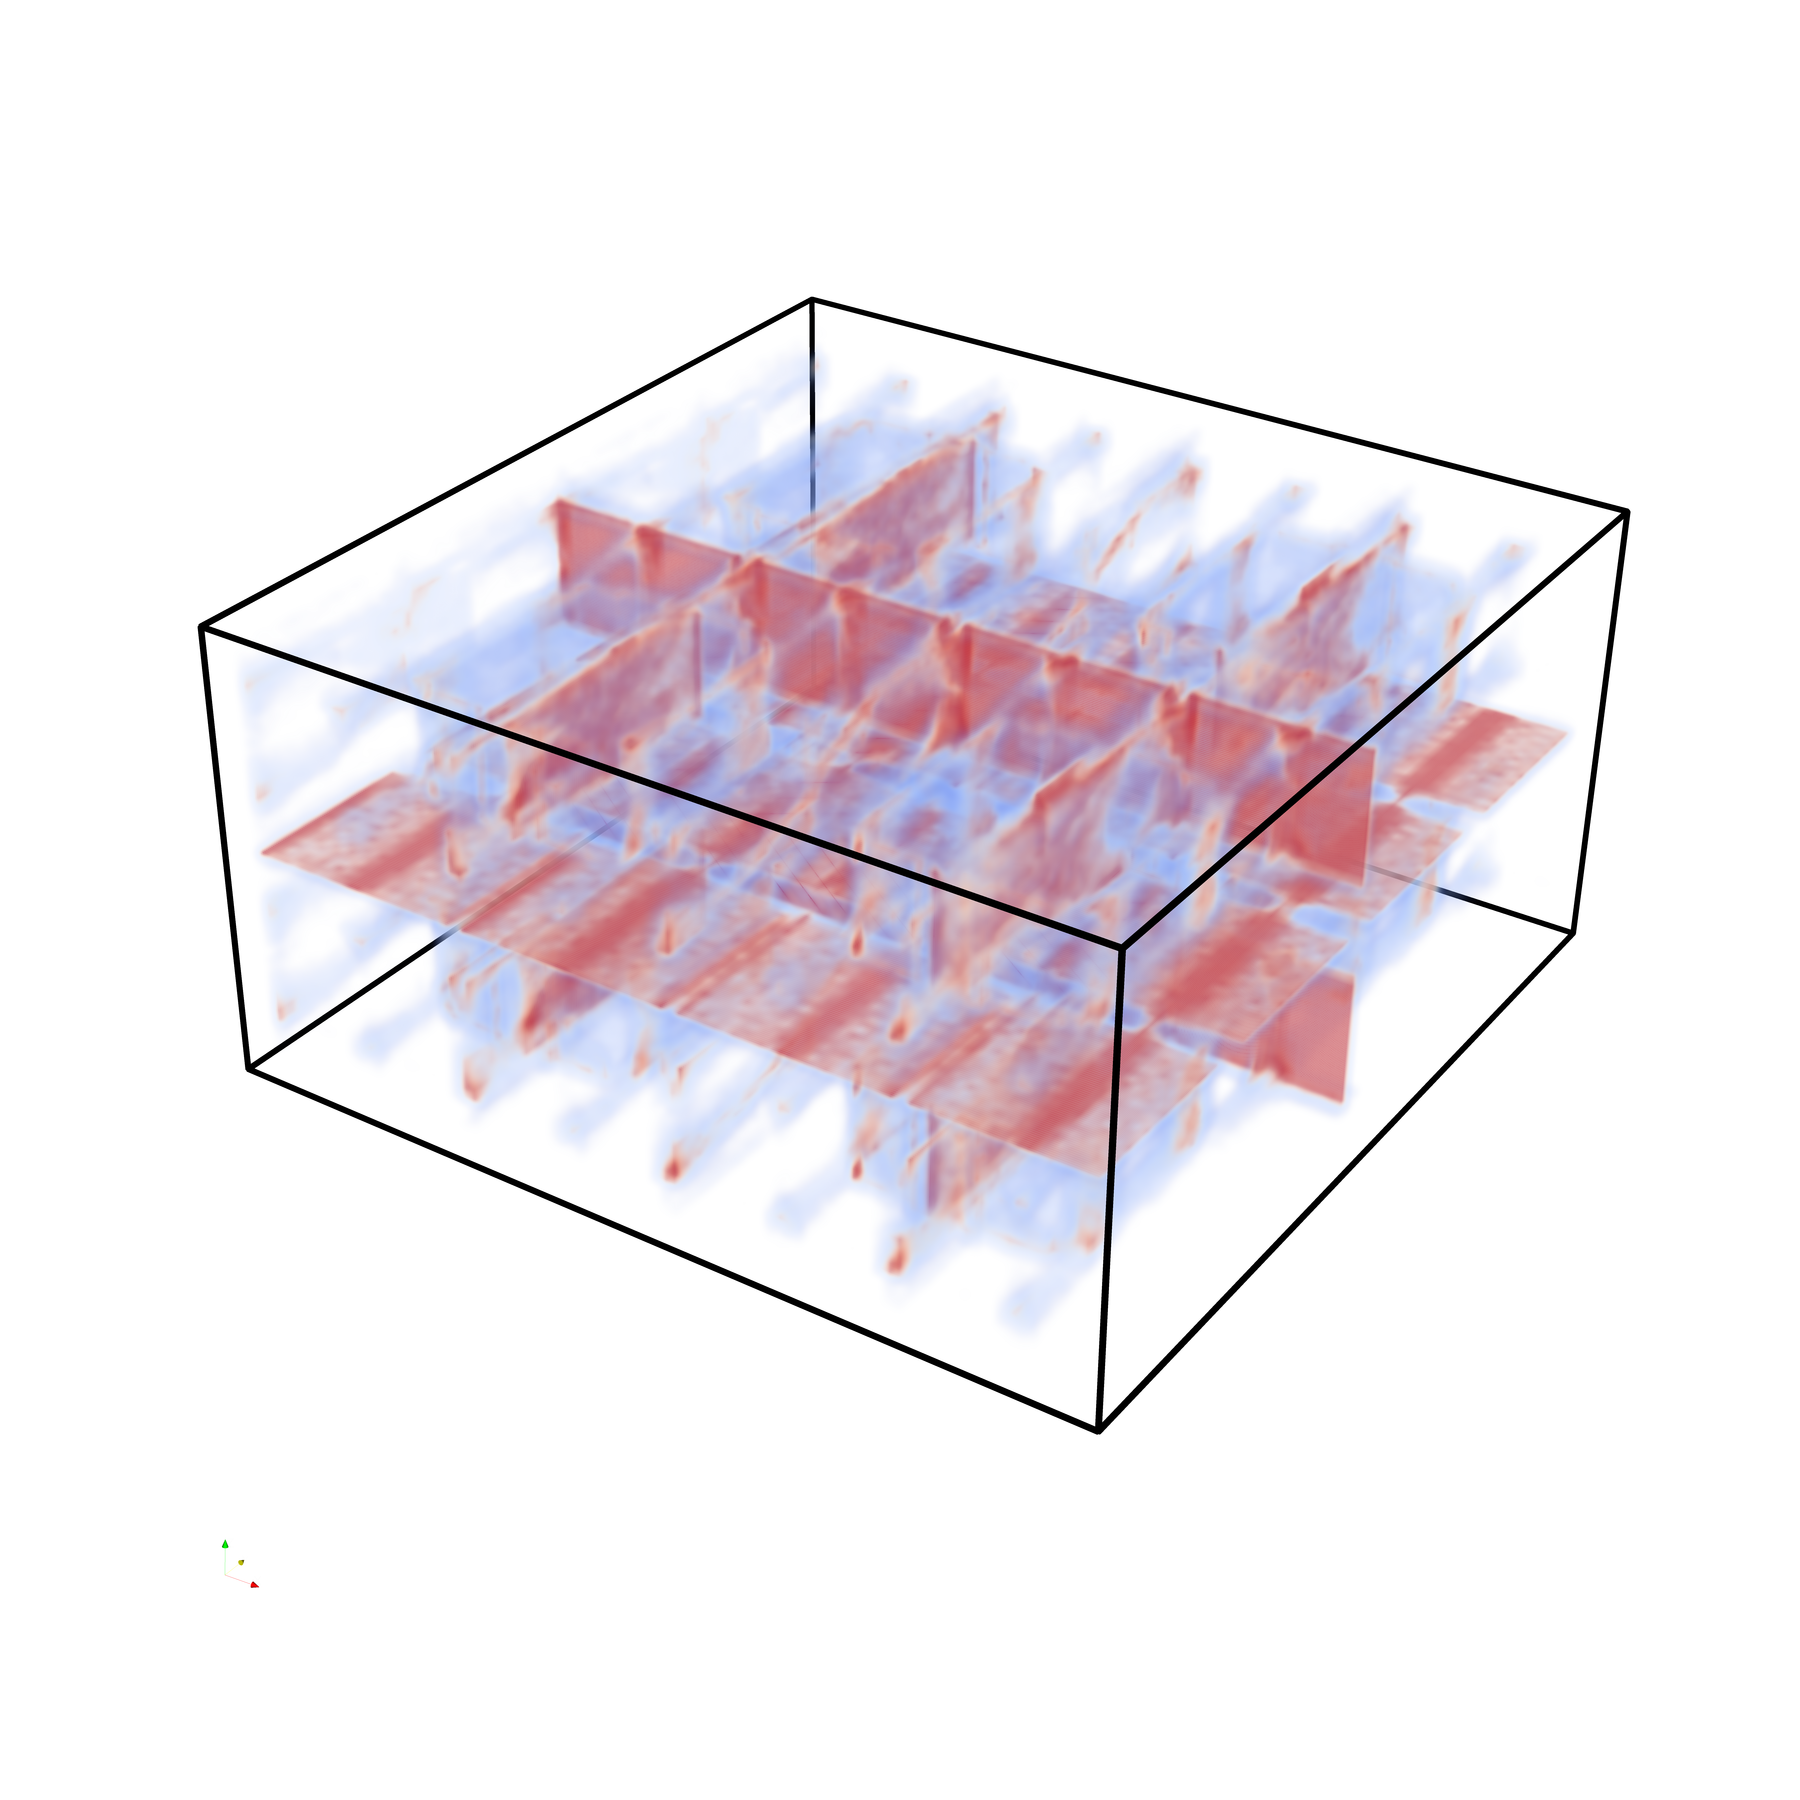
\includegraphics[width=\textwidth]{Images/shiftXoldchol.png}
        \caption{Cholesky}
        \label{fig:MCchol}
    \end{subfigure}
    \caption{Comparison of matrix decompositions for the uncertain
    ridge extraction using the Marching Cubes algorithm.}
    \label{fig:MCcomp}
\end{figure}

\begin{figure}
    \begin{subfigure}[b]{0.49\textwidth}
        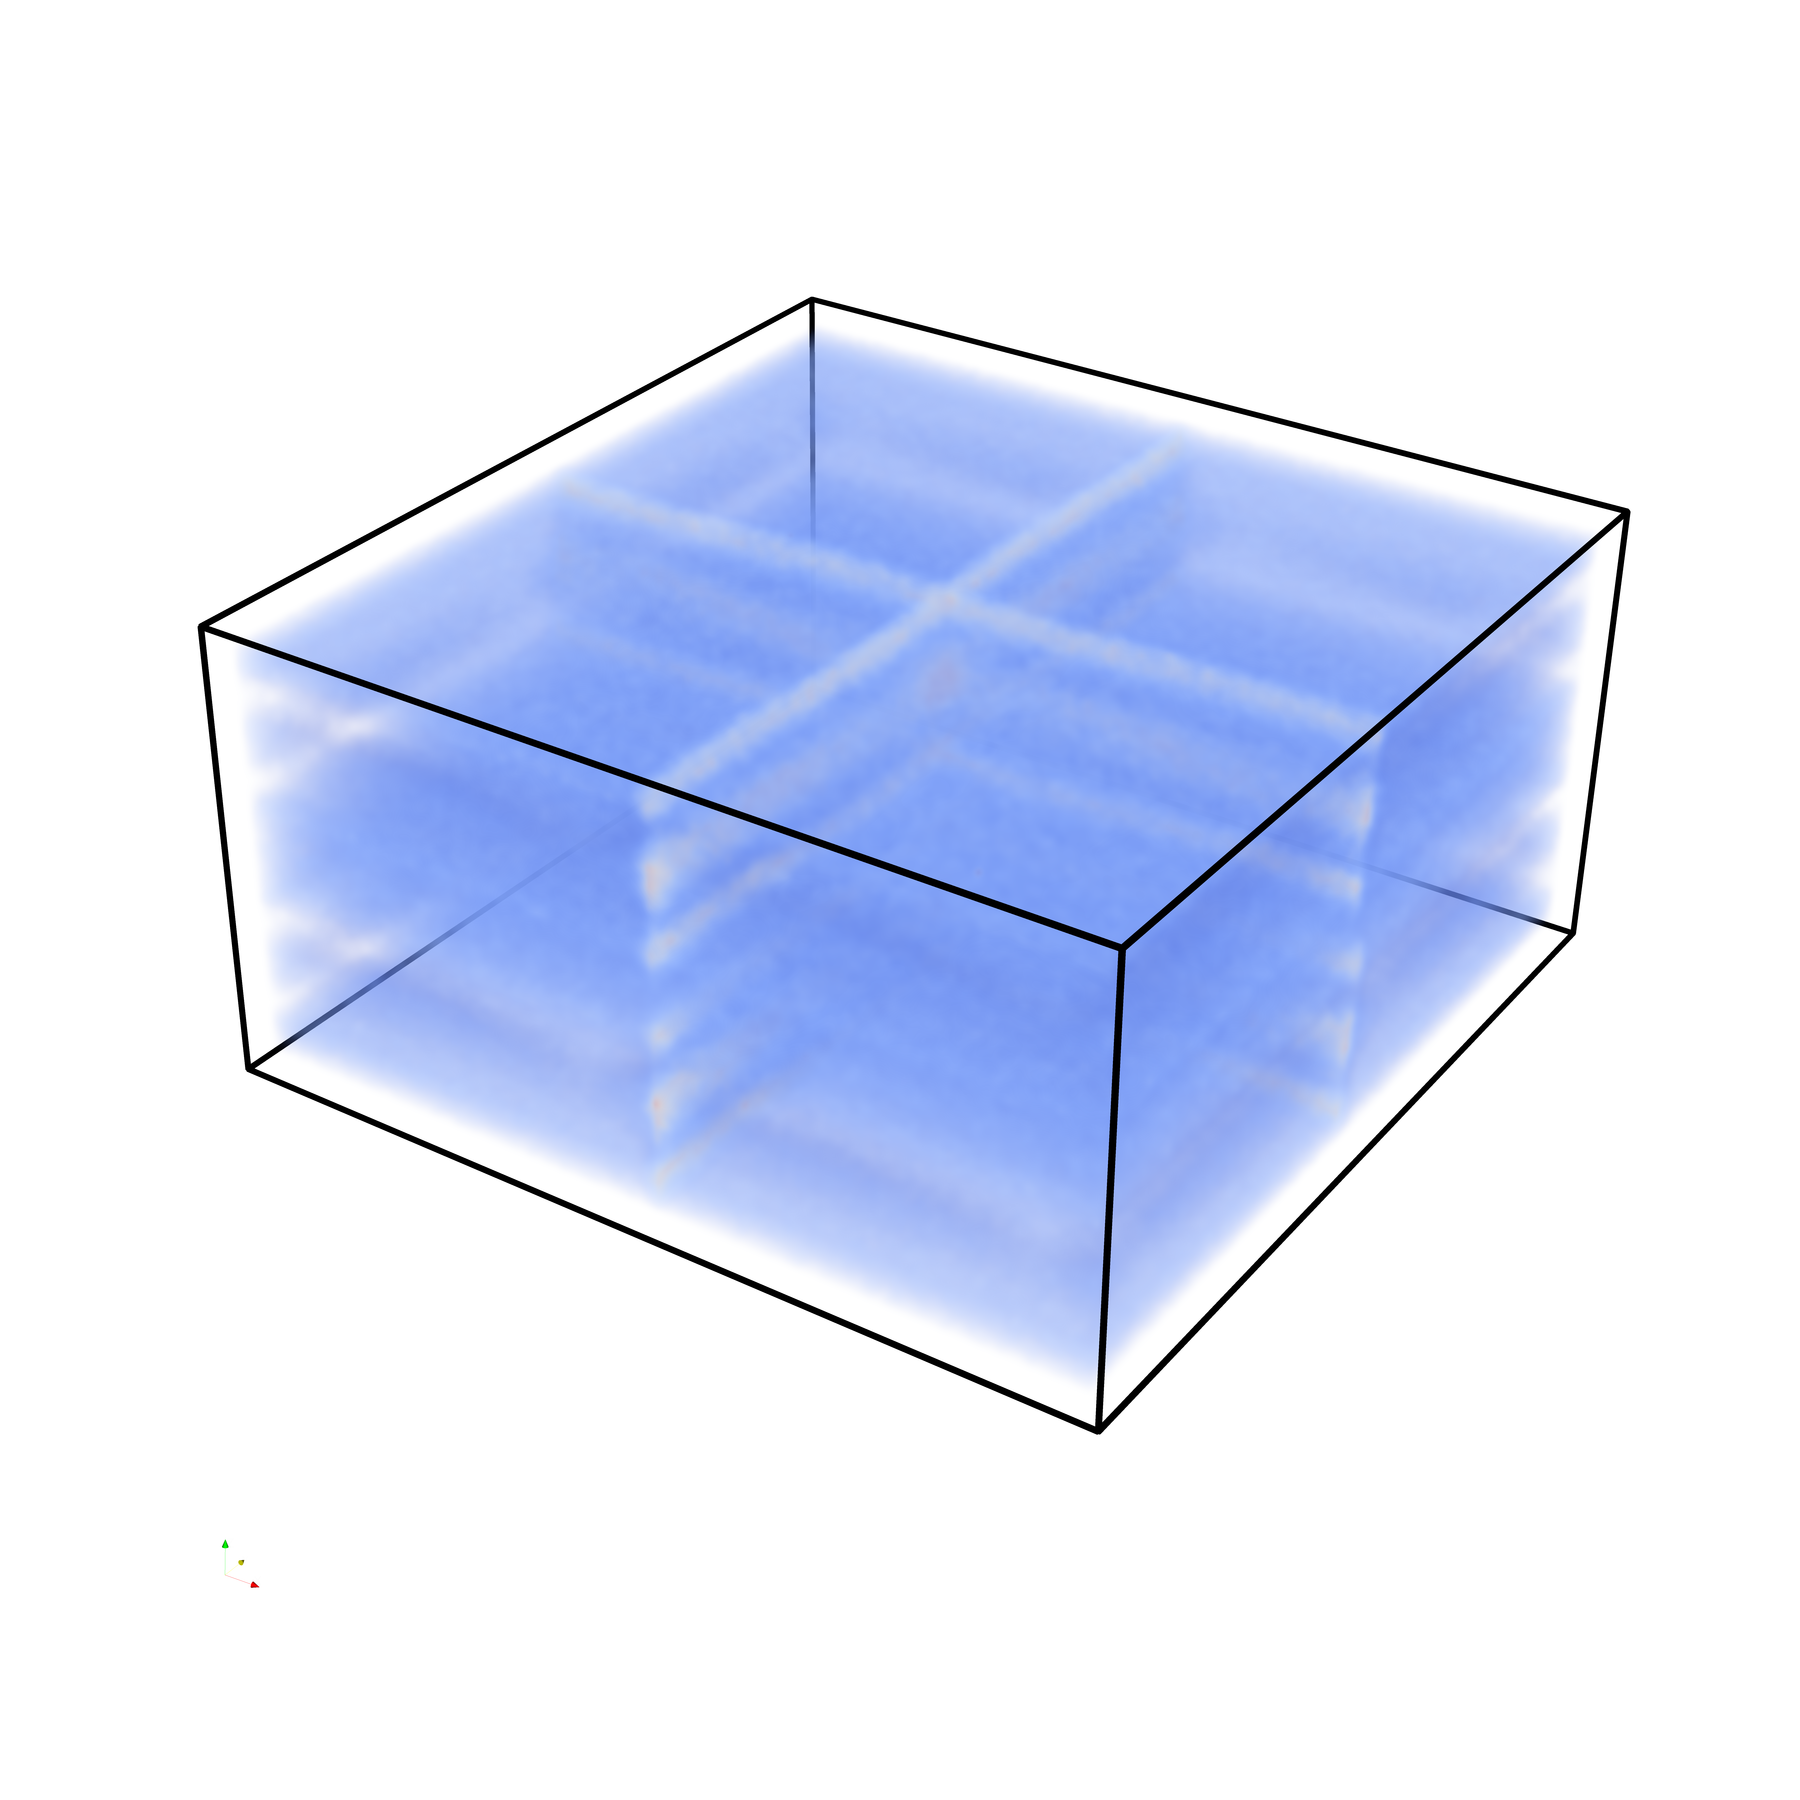
\includegraphics[width=\textwidth]{Images/highuncEigen.png}
        \caption{Eigendecomposition}
        \label{fig:HUCeigen}
    \end{subfigure}
    \begin{subfigure}[b]{0.49\textwidth}
        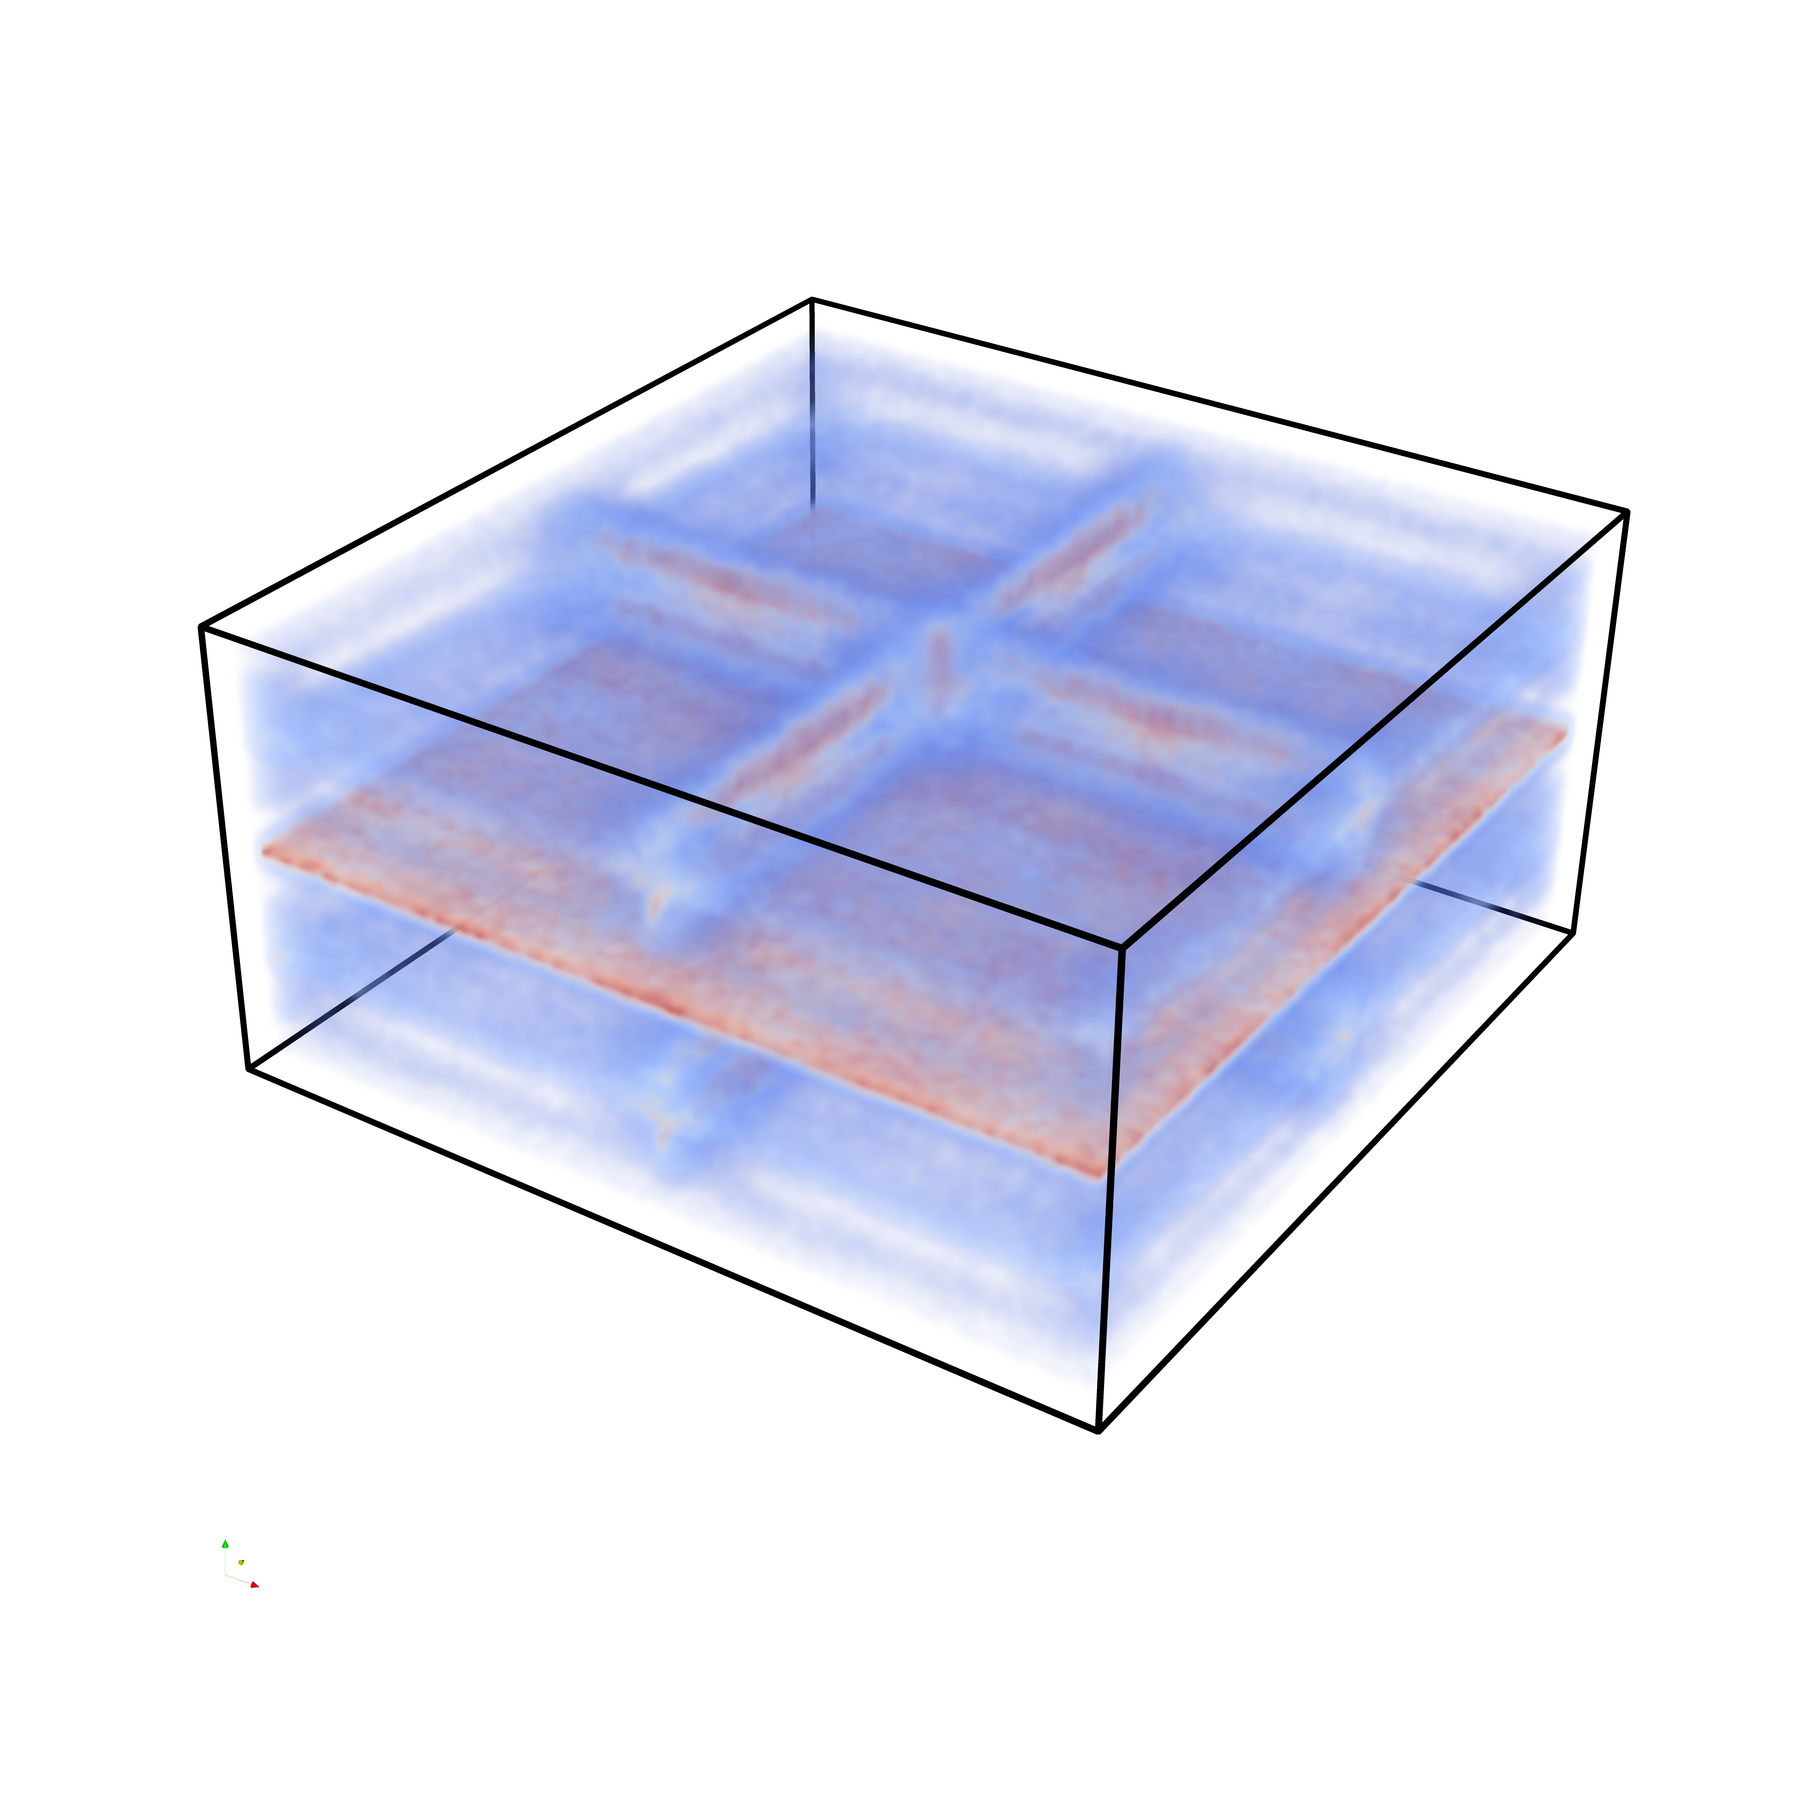
\includegraphics[width=\textwidth]{Images/highuncChol.png}
        \caption{Cholesky}
        \label{fig:HUCchol}
    \end{subfigure}
    \caption{Comparison of matrix decompositions for a set with high
    variance in every dimension. The Eigendecomposition exhibits a ridge
    structure appearing roughly around the mean, hardly distinguishable 
    from the noise surrounding it. Cholesky delivers a more certain
    structure, with holes in the cross like ridges on top and bottom,
    due to the up and downward distortion of the members.}
    \label{fig:HUCcomp}
\end{figure}
  %%%%%%%%%%%%%%%%%%%%%%%%%%%%%%%%%%%%%%%%%%%%%%%%%%%%%%%%%%%%%%%%%%%%%%%%
\chapter{Discussion}
%%%%%%%%%%%%%%%%%%%%%%%%%%%%%%%%%%%%%%%%%%%%%%%%%%%%%%%%%%%%%%%%%%%%%%%%

Pipapo Diskutieren.
}
% This ensures that the subsequent sections are being included as root
% items in the bookmark structure of your PDF reader.
\bookmarksetup{startatroot}
\backmatter{
  \printindex
  \printglossary{}
  \printbibliography{}
}
\end{document}
